\chapter{Elements of Audio Signal Processing}\label{ch:processing}
\openepigraph{Signal, a function that conveys information about a phenomenon.
$[\dots]$ Consider an acoustic wave, which can convey acoustic or music information.}{R. Priemer, \textit{Introductory Signal Processing}}
\vspace{-2.5em}
\newthought{Synopsis} Let us now move from the physics to digital signal processing.
At first this chapter formalized fundamental concepts of audio signal processing such as signal, mixtures and noise~\cref{sec:processing:model}.
Secondly, this concepts representation~\cref{sec:processing:domains}
The notation and the material presented in this chapter are inspired and extracted from~\citeauthor{vincent2018audio}'s book \textit{Audio source separation and speech enhancement}.

\section{Signal model in the time domain}\label{sec:processing:model}
In the previous chapter we formalized the physics that rule the sound propagation from the source 'till the microphone.
A raw \textit{audio signal} encodes the variation of pressure over time on the microphone membrane.
Mathematically it is denoted as the function
\begin{center}
    $\contTime{\mic}\in\bbR$
    ,
\end{center}
continuous both in time $t \in \R$ and amplitudes.
\marginpar{
    \centering
    \footnotesize
    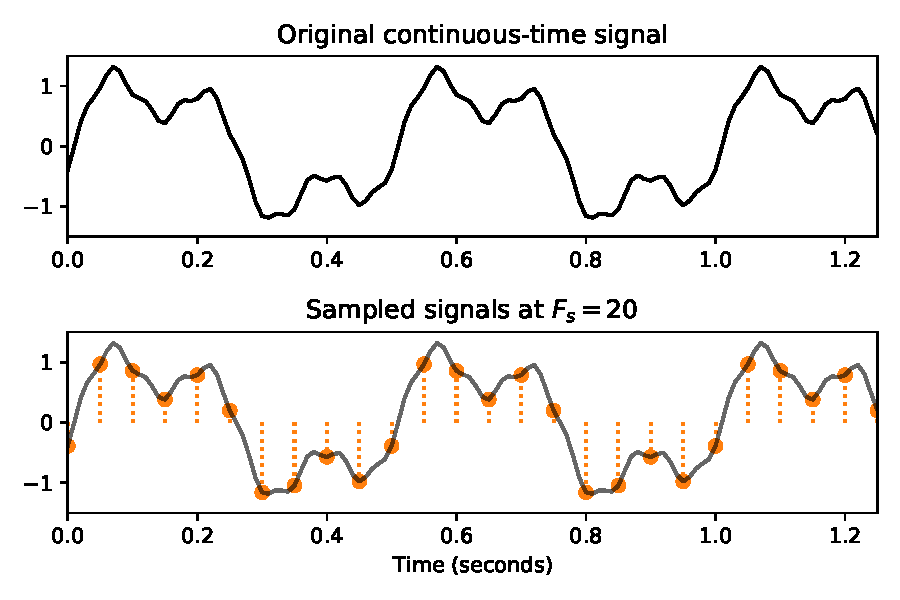
\includegraphics[width=\linewidth]{processing/py_processing.pdf}
    \captionof{figure}{Continuous-time signal and its sampled version.}
    \label{fig:processing:sampling}
}

Today signals are processed, stored and analyzed by computers and modules as \textit{digital audio signal}:
\begin{center}
    $\discTime{\mic}\in\bbR$
    ,
\end{center}
with discrete value in time $n \in \Z$.
In short, the digital representation is obtained from an analog signal in two steps:
first, the continuous time signal is \textit{sampled}\sidenote{
   Please note, that the use of the word \textit{sample} will have different
   meanings in the context of machine learning, where a sample is an instance of a full signal instead of a single time
}
at the \textit{sampling rate},  $\Fs$ in $[\si{\Hz}]$;
secondly, the amplitude values can be \textit{quantized}.
At the end of the digitalization, $x[n] \in \R$ with $n = 0, \dots, N-1$, represents a one dimensional finite time series of amplitudes.

The sampling can be modeled as a two-stage process:
first, the continuous-time signal undergoes a (ideal) low-pass filter $\lowpassfilter$\sidenote{
    The low-pass filter is used to reduce aliasing by removing spectral components higher than Fs.
    $\lowpassfilter(t) = \sinc(t) = \sin(\pi t) / (\pi t)$.
} with frequency support in $\kintervoc{\sfrac{-\Fs}{2}}{\sfrac{\Fs}{2}}$, limiting the signal frequencies to at max $\sfrac{\Fs}{2}$;
secondly, it is regularly sampled at rate $\Fs$.
This processes can be written in one equation:
\begin{equation}
    x[n] = (\lowpassfilter \conv x)\kparen{\frac{n}{\Fs}}
    \mathspace
    \kforall[n = 0, \cdots, N-1]
    ,
\end{equation}
where $\conv$ is the continuous-time convolution operator.

The choice of $\Fs$ depends on the application since it is a trade-off between computational power, processing and rendering quality.
Historically the two iconic values are $\SI{44.1}{\kHz}$ for music distribution on CDs and $\SI{8}{\kHz}$ for first-generation speech communication.
Now multiple of $\SI{8}{\kHz}$ are typical used in audio processing: ($16, 48, 96, \SI{128}{\kHz}$).
\\For further details, we refer the reader to audio signal processing basics books such as~\citeonly{rocchesso2003introduction}.

\mynewline
Audio signals are emitted by sources and are observed, received or recorded by microphones.
A set of microphones is called a microphone \textit{array}, whose signals are sometime referred to as \textit{channels}.
In this thesis, these objects are assumed to have been deployed in a indoor environment, called generically \textit{room}.
% \begin{center}
%     \textit{All of these make our indoor \emph{auditory scene}.}
% \end{center}
Let us provide some taxonomy, through some dichotomies, useful for describe the mixing process later:

\dichotomy{Sources \vs/ Mixtures:}
Sound sources emits sounds.
When multiple sources are active at the same time, the sound that reaches our ears or is recorded using a microphone is superimposed or \textit{mixed} to a single sound.
This resulting signal is denoted as \textit{mixture}.

\dichotomy{Single-Channel \vs/ Multichannel:}
The term \textit{channel}\sidenote{%
    Please note, the term \textit{channel} has also different meaning:
    it indicates the medium in communication (\eg/ Channel Estimation)
    and sometimes one of the dimension of the input in machine learning (\eg/ image's channel).
} is used here to indicate the output of one microphones or one source.
A \textit{single-channel} signal ($\numMics = 1$) is represented by the scalar $\mic(t) \in \R$,
while a \textit{multichannel} ($\numMics >   1$) is represented by the vector $\mics(t) = \ktranspose{\klist{\mic_1(t), \dots, \mic_{\numMics}(t)}} \in \R^{\numMics}$.

\dichotomy{Point \vs/ Diffuse Sources:}
\textit{Point sources} are emitted by a single and well-defined point in the space and their signal is single-channel.
Point sources are for instance human speakers or the sound emitted by a loudspeaker.
\\\textit{Diffuse sources} refers for instance to wind, traffic noise, or large musical instruments, which emit sound in a large region of space.
Their sound cannot be associate to a punctual source, but rather a distributed collection of them.

\dichotomy{Directional \vs/ Onmidirectional:}
An \textit{omnidirectional} source (\resp/ receiver) will in principle emit (\resp/ pick up) sound equally from all directions,
both in time and in frequency.
Although this simplify greatly processing models and frameworks, this is not true in real scenario.
The physical properties of real sources (\resp/ receivers) leads to \textit{directivity patterns}, \aka/ \textit{polarity}, which may
be different at different frequencies.
In this thesis we will assume always omnidirectional sources and receivers.
% This effect may be a source of undesired effects, such as microphones \textit{leakage} or source localization error.
% Nevertheless sometimes it can be exploited to promote \textit{spatial selectivity}:
% spatial filtering can be view under this light, where ``virtual'' microphones with engineered directivity pattern.

\subsection{The Mixing Process}
Let us assume the observed signal has $\numMics$ \textit{channels} indexed by $\idxMic \in \kbrace{1,\dots,\numMics}$.
Let us assume that there are $\numSrcs$ sources indexed by $\idxSrc \in \kbrace{1,\dots,\numSrcs}$.
Each microphone $\idxMic$ and each source $\idxSrc$ have a well defined position in the space, $\positionMicrophone_\idxMic$, $\positionSource_\idxSrc$, respectively.

The mixing process describes then the nature of the mixtures.
In order to better formalized it, \citeauthor{sturmel2012linear} introduced the intermediate representation called \emph{source spatial images}:
\begin{center}
    \textit{$\img_{\idxMic\idxSrc}(t)$ describes the contribution of the source $\idxSrc$ to the microphone $\idxMic$}.
\end{center}
Consequently, the \textit{mixture} $\mic_{\idxSrc}(t)$ is the possibly non-linear combination of images associated to the source $j$.
Depending on the ``contribution'' the image describes, the following type of mixture can be defined:

\dichotomy{Natural \vs/ Artificial Mixtures:}
The former refers to microphone mixtures recorded simultaneously the same auditory scene, \eg/ teleconferencing systems or hands-free devices.
By contrast, the latters are created by mixing together different individual, possibly processed, recordings.
This are the typical mixtures used professional music production\sidenote{here the usage of long-chain of audio effects typically ``hide'', willingly or not, the recording environment of the sound sources}.

\dichotomy{Instantaneous \vs/ Convolutive Mixtures:}
In the fist case, the mixing process boils down to a simple linear combination of the source signals, namely
the mixing filters are just scalar factors.
This is the typical scenario when sources are mixed using a mixing console.
\marginpar{%
    \footnotesize
    \centering
    \begin{tabular}{p{0.33\linewidth}|p{0.66\linewidth}}
    \toprule
    instantaneous   & $x_{i} \ =\sum ^{J}_{j=1} a_{ij} s_{j} $ \\
    anechoic        & $x_{i} \ =\sum ^{J}_{j=1} a_{ij} s_{j}( t - \tau _{ij}) $ \\
    convolutive     & $x_{i} \ =\sum ^{J}_{j=1}( g_{ij} \ast s_{j})( t)$ \\
    \bottomrule
    \end{tabular}
    \captionof{table}{Taxonomy of linear mixing models for a mixture channel $x_i$, sources $s_j$, impulse response $g_{ij}$,
    scaling factor $a_{ij}$ and delay $\tau_{ij}$.}
}
Convolutive mixtures, instead, denote the more general case where the each mixture is the sum of filtered signals.
In between are the \textit{anechoic} mixtures involving the sum of scaled and delayed source signals.
Natural mixtures are convolutive by nature and ideal free-far-field natural recording are well approximated by anechoic mixtures.

% Being $\spat_\idxSrc(\cdot)$ a possibly nonlinear spatialization operation, the spatial images
% $\imgs_\idxSrc(t) = \ktranspose{\klist{\img_{1\idxSrc}(t), \dots, \img_{\numMics\idxSrc}(t)}}$ with respect to the $\numMics$ reads
% \begin{equation}
%     \imgs_\idxSrc(t) = \kbracket{\spat_\idxSrc(\idxSrc)}(t)
%     .
% \end{equation}
% In second stage, the images of all (point and diffuse) sources are added together and passed through a possibly
% nonlinear \textit{post-mixing} operation $\master(\cdot)$ to obtain the mixture signal $\mics(t)$
% \begin{equation}
%     \mics(t) = \kbracket{ \master\kparen{
%                     \sum_{\idxSrc=1}^{\numSrcs} \imgs_\idxSrc
%                     }}(t)
% \end{equation}
% \marginpar{
%     \footnotesize
%     In the field of music productions,
%     $\spat_\idxSrc(\cdot)$ and $\master(\cdot)$ may be identify rispectively with the \textit{mixing} and \textit{mastering} process.
% }

\begin{figure}[t]
    \begin{fullwidthfig}
        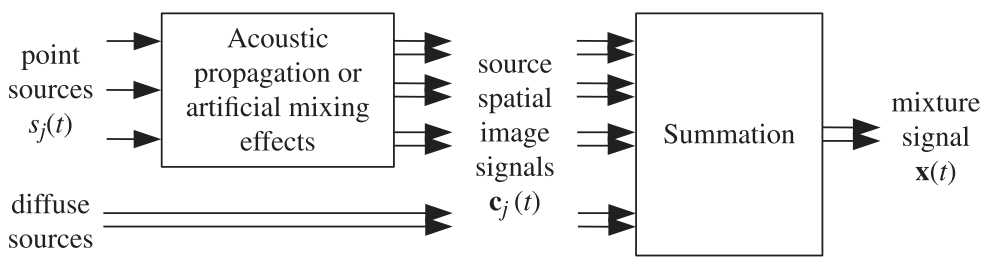
\includegraphics[width=\linewidth+\marginparsep]{processing/mixing_process.png}
    \end{fullwidthfig}

    \vspace{-\baselineskip}\vspace{-\baselineskip}
    \sideparmargin{outer}
    \sidepar{\vspace{\baselineskip}
    \caption{General mixing process, illustrated in the case of $\numSrcs = 3$ sources,
      including three point sources and one diffuse source, and $\numMics = 2$ channels.}
    }
    \label{fig:processing:mixing}
\end{figure}

\newthought{In this thesis}, we will particularly focus on natural mixture:
the microphone mixture listens to the propagation of sound in the room and this process is linear (\cfr{\cref{ch:acoustics:sec:wave}}) and time invariant provided a static scenario.
% In this case, the spatialization operation $\spat_\idxSrc(\cdot)$ is expressed by
% collection of convolution with \RIR/ $h_{\idxMic\idxSrc}$
% from source $\idxSrc$ to microphone $\idxMic$ and the post-mixing operation $\master(\cdot)$ reduces to the identity:
Therefore, the resulting mixture is the simple summation of the sound images,
which are the collections of convolution between the \RIRs/ and source signal:
\marginpar{
    \centering
        \tikzset{every picture/.style={line width=0.75pt}} %set default line width to 0.75pt
        \resizebox{\linewidth}{!}{
            \begin{tikzpicture}[x=0.75pt,y=0.75pt,yscale=-1,xscale=1]

                % Picture Node
                \draw (333,148.65) node  {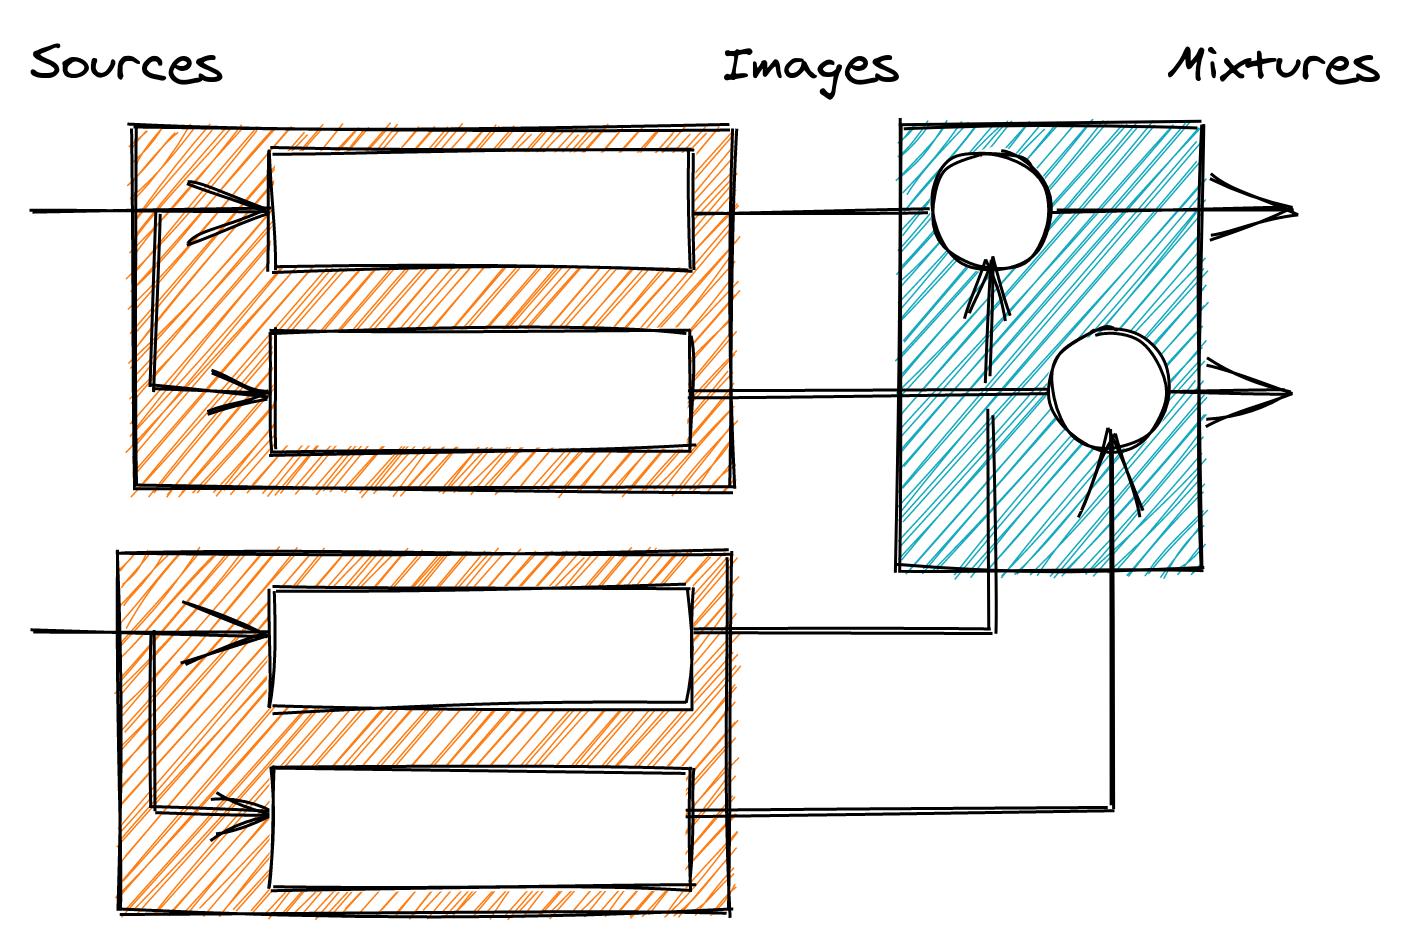
\includegraphics[width=333.75pt,height=222.97pt]{processing/mixing_blocks.png}};

                % Text Node
                \draw (126,53) node [font=\huge]   {$s_{1}$};
                % Text Node
                \draw (126,183) node  [font=\huge]  {$s_{2}$};
                % Text Node
                \draw (262,63) node  [font=\huge]  {$h_{11} \ast s_{1}$};
                % Text Node
                \draw (262,120) node  [font=\huge]  {$h_{21} \ast s_{1}$};
                % Text Node
                \draw (370,53) node  [font=\huge]  {$c_{11}$};
                % Text Node
                \draw (370,110) node [font=\huge]   {$c_{21}$};
                % Text Node
                \draw (530,53) node   [font=\huge] {$x_{1}$};
                % Text Node
                \draw (530,110) node  [font=\huge]  {$x_{2}$};
                % Text Node
                \draw (262,199) node  [font=\huge]  {$h_{12} \ast s_{2}$};
                % Text Node
                \draw (262,256) node  [font=\huge]  {$h_{22} \ast s_{2}$};
                % Text Node
                \draw (370,183) node  [font=\huge]  {$c_{12}$};
                % Text Node
                \draw (370,240) node   [font=\huge] {$c_{22}$};
                % Text Node
                \draw (412,53) node [anchor=north west][inner sep=0.75pt]  [font=\huge]  {$\sum $};
                % Text Node
                \draw (448,109) node [anchor=north west][inner sep=0.75pt]  [font=\huge]  {$\sum $};

            \end{tikzpicture}
        }
        \captionof{figure}{Graphical representation of the mixing model~\ref{eq:processing:mixing:mix} for 2 sources and 2 microphones.}\label{fig:processing:mixing}
}
\begin{align}
    \img_{\idxMic\idxSrc}(t) &=  \kparen{h_{\idxMic\idxSrc} \conv \src_\idxSrc} (t)     \label{eq:processing:mixing:img} \\
    \imgs_\idxSrc(t) &= \ktranspose{\klist{\img_{1\idxSrc}(t), \dots, \img_{\numMics\idxSrc}(t)}} \nonumber\\
    \mics(t)         &= \sum_{\idxSrc=1}^{\numSrcs} \imgs_\idxSrc(t)                    \label{eq:processing:mixing:mix}
    .
\end{align}%
Considering the time domain description of the \RIR/ derived (and approximated) in the previous chapter,
the time-domain \emph{mixing filters} $h_{ij}( t)$ will be modeled as follows:
\begin{equation}\label{eq:processing:mixing_filter}
    h_{ij}( t) = \sum_{\idxEch=0}^{\numEchs} \frac{\absCoeff_{ij}^r}{4 \pi \speedOfSound \tau_{ij}^r}
                       \diracOf{t - \tau_{ij}^r} + \varepsilon_{ij}(t)
\end{equation}
where $\absCoeff_{ij}^r$ and $\tau_{ij}^r$ are the attenuation coefficient and the time delay of the reflection $\idxEch$.
The noise term $\varepsilon_{ij}( t)$ collects later echoes ($\idxEch > \numEchs$) and the tail of the reverberation.
We do not assume $\varepsilon_{ij}( t)$ to be known.

\subsection{Noise, interferer and errors}
% \openepigraph{%
%     \emph{Noise} is a general term for unwanted (and, in general, unknown) modifications that a signal may suffer during capture, storage, transmission, processing, or conversion
% }{V. Tuzlukov, \textit{Signal processing noise}}
In~\cref{eq:processing:mixing:mix} no noise is included:
all the sources are threated in the same way, including \textit{target}, \textit{interfering} and \textit{noise} sources.
While the definition of target sound source is quite self-explanatory and it will denoted by default as the first source, that is $j = 1$,
the term interfer and noise depends on the specific use case, problem, application, and research field.
Notice that in~\cref{eq:processing:mixing_filter} a noise term is added to gather unknown quantities.
\begin{quote}
    \textit{\emph{Noise} is a general term for unwanted (and, in general, unknown) modifications that a signal may suffer during capture, storage, transmission, processing, or conversion}
    \citeonly{tuzlukov2018signal}.
\end{quote}
Therefore, we will define and use the following type of noises:
\marginpar{
    \centering
        \resizebox{\linewidth}{!}{
            \begin{tikzpicture}[x=0.75pt,y=0.75pt,yscale=-1,xscale=1]
            \draw (346.67,226.03) node  {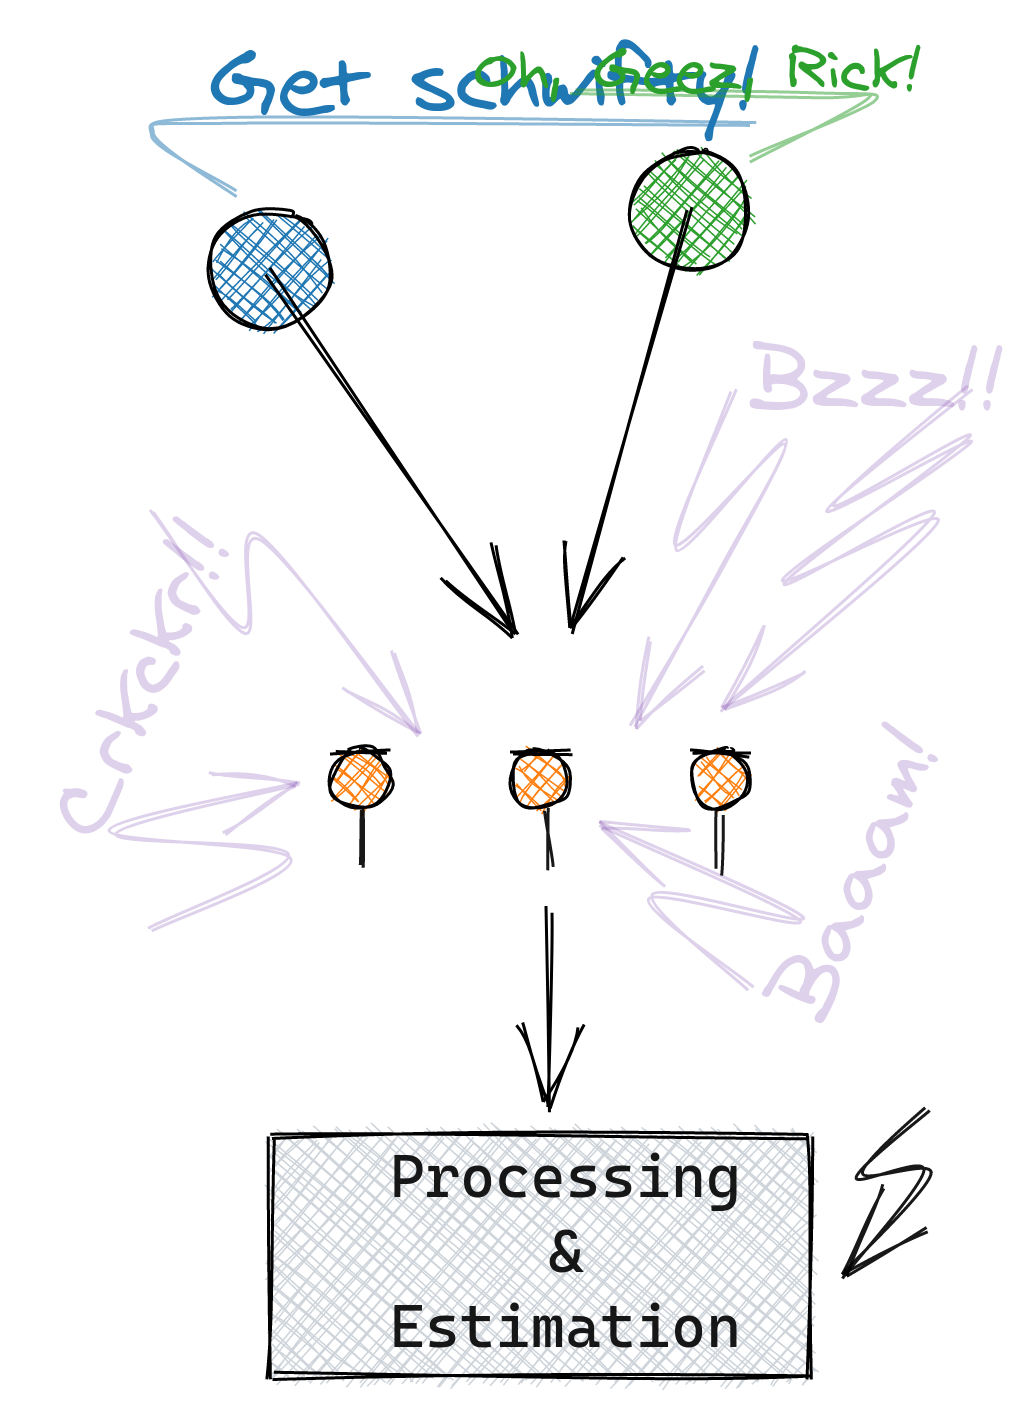
\includegraphics[width=246.25pt,height=335.73pt]{processing/noise.png}};
            % Text Node
            \draw (203.5,100.4) node [anchor=north west][inner sep=0.75pt]  [font=\Large]  {$s_{1}( t)$};
            % Text Node
            \draw (429.5,49.9) node [anchor=north west][inner sep=0.75pt]  [font=\Large]  {$s_{2}( t)$};
            % Text Node
            \draw (455.5,196.9) node [anchor=north west][inner sep=0.75pt]  [font=\Large]  {$\boldsymbol{n}( t)$};
            % Text Node
            \draw (308.5,285.9) node [anchor=north west][inner sep=0.75pt]  [font=\Large]  {$\boldsymbol{x}( t)$};
            % Text Node
            \draw (465.5,327.4) node [anchor=north west][inner sep=0.75pt]  [font=\Large]  {$\boldsymbol{\varepsilon }( t)$};
            \end{tikzpicture}
        }
        \captionof{figure}{Graphical representation of the mixing model~\eqref{eq:processing:mixing:mix}:
        $s_2(t)$ is the \textit{interferer},
        $\boldsymbol{n}( t)$ contributes to the \textit{diffuse noise field}, and
        $\boldsymbol{\varepsilon }( t)$ model acquisition and modeling errors.
        }\label{fig:processing:mixing}
}
\newthought{Interfers} identifies the undesired source with properties similar to the target source.
For instance, a concurrent speech source for speech application or concurrent music instrument in case of music.
\\In this thesis, and in particular in~\cref{ch:dataset,ch:brioche}, the interfer sources will be denoted
as additional source indexed by $j > 1$.
\newthought{Noise} collects all the remaining effects, typically nonspeech sources. Moreover we will make a further distinction between the followings.

\newthought{Diffuse Noise Field} describes the background diffuse sources present in the auditory scene, \eg/ car noise, indistinct talking or winds.
It can be recorded or approximated as \AWGN/ with a specific spatial description~\citeonly{habets2007generating}.
% \\In this thesis, it is denoted as $\bsn(t) \sim \calN(0, \cov_{nn})$ where $\cov_{nn} \in \bbR^{I \times I}$ is the noise \textit{spatial covariance matrix}

\newthought{Measurement and Model Noise} accounts for general residual miss- and under-modeling error.
As common is signal processing and information theory, this error term will be modeled as \AWGN/.
\\In this thesis, it will denoted as $\varepsilon_{ij}( t)$ and will be used to model the
approximation of the \RIR/ with the \ISM/ or sensor noise, respectively.

\mynewline
By making the noisy terms explicit, the mixing model in~\cref{eq:processing:mixing:img,eq:processing:mixing:mix} writes:
\begin{align}
    \img_{\idxMic\idxSrc}(t) &=  \kparen{h_{\idxMic\idxSrc} \conv \src_\idxSrc} (t) +  \varepsilon_{ij}(t)\\
    \imgs_\idxSrc(t)         &= \ktranspose{\klist{\img_{1\idxSrc}(t), \dots, \img_{\numMics\idxSrc}(t)}} \nonumber\\
    \mics(t)                 &= \sum_{\idxSrc=1}^{\numSrcs} \imgs_\idxSrc(t) + \bsn( t)
\end{align}

% $\bsu = \bsn + \boldsymbol{\varepsilon}$

\section{Signal Model in the Spectral domains}\label{sec:processing:domains}

The frequency, or spectral, representation is probably the most famous signal representation used in signal processing\sidenote{%
It was introduced by Joseph Fourier in his work on the heat equation~\citeonly{fourier1822theorie}.
His mathematical tool, named later \textit{Fourier Decomposition},
aims at approximating any signal by a sum of sine and cosine waves.}:
Speech and music signals naturally exhibit harmonic and periodic behaviors and
through it are described as combination of sinusoids as function of their frequencies.
% https://tex.stackexchange.com/questions/127375/replicate-the-fourier-transform-time-frequency-domains-correspondence-illustrati

This operation is achieved by the \FTdef/, $\fourierTrans{}:\bbR\kmapsto\bbC$, which projects a continuous-time-domain signal $x$ onto a space spanned by continuous-frequency complex exponentials:
\begin{equation}\label{eq:processing:ft}
    x(f) = (\fourierTrans{x})(f) =
        \int_{-\infty}^{+\infty}
        x(t)
        \cste^{-\csti 2 \pi f t}
        \,\kdiff{t}
    ,
\end{equation}
where $f \in \bbR$ are the \textit{natural frequency} in $\si{\Hz}$ and $\csti$ is the imaginary unit.

\marginpar{

    %define colors
    \definecolor{lightgray}{rgb}{0.8, 0.8, 0.8} %grid of coordinate system, axes
    \definecolor{midgray}{rgb}{0.6, 0.6, 0.6} %layer of border
    \definecolor{darkgray}{rgb}{0.4, 0.4, 0.4} %curves, fill under curve

    \centering
    \resizebox{\linewidth}{!}{

        \begin{tikzpicture} %create tikz picture
        \begin{axis}[ %create 3d plot within tikz
            set layers=standard, %use predefined layers
            view={50}{30}, %perspective adjustment
            domain=0:10, %plot limit in time direction
            samples y=1, %samples for frequency direction
            unit vector ratio*=1 2 1, %rescale unit vectors
            hide axis, %do not plot axes
            xtick=\empty, ytick=\empty, ztick=\empty, %no ticks on coordinate axes
            clip=false %let me plot outside the coordinate system
        ]
            %limit variables
            \def\xmax{100} %limits for curves and layers
            \def\xmin{0}
            \def\ymax{35}
            \def\ymin{5}
            \def\zmax{25}
            \def\zmin{-5}
            \def\xlayer{110} %frequency layer
            \def\sumcurve{0} %sum curve of time signal

            %frequency curves
            \pgfplotsinvokeforeach{1,2,3}{ %for each frequency component
                \draw [on layer=background, lightgray] (axis cs:0,#1,0) -- (axis cs:10,#1,0); %axes
                \addplot3 [on layer=main, darkgray, smooth, samples=200] (x,#1,{1.3*sin(2*#1*x*(157))/(#1*2)}); %plot curves (curves are somewhat arbitrary)

                \xdef\sumcurve{\sumcurve + sin(#1*x*(157))/(#1*2)} %add current curve to sumcurve
            }

            %transparent layers
            \fill[white,opacity=0.7] (\xmin,0,\zmin) -- (\xmin,0,\zmax) -- (\xmax,0,\zmax) -- (\xmax,0,\zmin) -- cycle; %transparent layer in time space
            \fill[white,opacity=0.7] (\xlayer,\ymin,\zmin) -- (\xlayer,\ymin,\zmax) -- (\xlayer,\ymax,\zmax) -- (\xlayer,\ymax,\zmin) -- cycle; % transparent layer for frequency space

            %grid lines
            \pgfplotsinvokeforeach{\xmin,\xmin+5,...,\xmax}{ %create horizontal grid lines (time layer)
                \draw[lightgray,opacity=0.6] (#1,0,\zmin) -- (#1,0,\zmax);
            }
            \pgfplotsinvokeforeach{\ymin,\ymin+2.5,...,\ymax}{ %create horizontal grid lines (frequency layer)
                \draw[lightgray,opacity=0.6] (\xlayer,#1,\zmin) -- (\xlayer,#1,\zmax);
            }
            \pgfplotsinvokeforeach{\zmin,\zmin+5,...,\zmax}{ %create vertical grid lines (both layers)
                \draw[lightgray,opacity=0.6] (\xmin,0,#1) -- (\xmax,0,#1);
                \draw[lightgray,opacity=0.6] (\xlayer,\ymin,#1) -- (\xlayer,\ymax,#1);
            }

            %borders layer
            \draw[midgray] (\xmin,0,\zmin) -- (\xmin,0,\zmax) -- (\xmax,0,\zmax) -- (\xmax,0,\zmin) -- cycle; %time space layer border line
            \draw[midgray] (\xlayer,\ymin,\zmin) -- (\xlayer,\ymin,\zmax) -- (\xlayer,\ymax,\zmax) -- (\xlayer,\ymax,\zmin) -- cycle; %frequency space layer border line

            %sum curve
            \addplot3 [samples=200] (x,0,{\sumcurve+rand/7+0.2*sin(x*400)}); %sum curve time space with added random noise

            % frequency curve
            \addplot3 [name path=f,samples=200,domain=0.5:3.5] (11,x,{rand/30+2*sin((x-0.7)*180)^200*e^(-x/2)-0.3}); %experimentally modified curve with noise

            %create fill under curve
            \addplot3 [name path=ax,draw=none,samples=2,domain=0.5:3.5] (11,x,-0.5); %create fill axis
            \addplot3 [darkgray] fill between [of=f and ax]; %create fill between curve and axis

            %create coordinate axis
            \draw[-{stealth}] (\xmin,0,\zmin-7) -- (\xmax/5.3,0,\zmin-7); %time axis
            \draw[-{stealth}] (\xlayer,\ymin,\zmin-7) -- (\xlayer,\ymin+\ymax/4,\zmin-7); %frequency axis

            %axis labels
            \node[scale=0.7] at (0,0,-21) {Time}; %axis time space
            \node[scale=0.7] at (100,22,-32) {Frequency}; %axis frequency space

        \end{axis}
        \end{tikzpicture}

        }
        % https://tex.stackexchange.com/questions/127375/replicate-the-fourier-transform-time-frequency-domains-correspondence-illustrati
        \captionof{figure}{
            A signals resolved into its Fourier series:
            a linear combination of sines and cosines
            represented as peaks in the frequency domain.
        }\label{fig:processing:mixing}
}

A part from providing a space where audio signal reveals their harmonic structures, the Fourier transforms benefits of two fundamental properties:
it is linear and it converts time-convolution into element products.
\\First, linearity allows to write~\cref{eq:processing:mixing:mix} simply as:
\begin{equation}\label{eq:processing:ft:mix}
    \mics( t) = \sum_{\idxSrc=1}^{\numSrcs} \imgs_\idxSrc( t)
    \;\overset{\fourierTrans{}}{\kto}\;
    \mics( f) = \sum_{\idxSrc=1}^{\numSrcs} \imgs_\idxSrc( f)
\end{equation}
Secondly, by the \textit{convolution theorem}, the source spatial images in~\cref{eq:processing:mixing:img} writes as:
\begin{equation}\label{eq:processing:conv}
    \img_{\idxMic\idxSrc}( t) =  \kparen{h_{\idxMic\idxSrc} \conv \src_\idxSrc} ( t)
    \;\overset{\fourierTrans{}}{\kto}\;
    \img_{\idxMic\idxSrc}( f) =  h_{\idxMic\idxSrc}( f) \src_\idxSrc( f)
    .
\end{equation}
As discussed in~\cref{chap:acoustics}, the \FT/ of a \RIR/ can be computed exactly in closed-form as
\begin{equation}\label{eq:processing:rir:ft}
    h_{ij}( f) = \sum_{\idxEch=0}^{\numEchs}
    \frac{\absCoeff_{ij}^r}{4 \pi \speedOfSound \tau_{ij}^r}
    \cste^{- \csti 2 \pi f \tau_{ij}^r}
    .
\end{equation}
In practice, the filters $h_{ij}$ are not available in the continuous time domain nor in the continuous frequency domain directly.
They can be estimated from the observation of the mixtures $x_i( n)$, therefore,
after the convolution with a source and the measurement process.
Notice that here both $f$ and $t$ are continuous and infinite variables.
In practice, we have access to finite and discrete-time microphones signals for which the properties~\eqref{eq:processing:conv} is valid with some precautions.

\subsection{Discrete frequency domain}
The spectral representation of a discrete-finite-time signal $x[n]$ is given by its (forward) \DFTdef/
\sidenote{
    % Please note that the notation for applying the \DFT/ is the one used for matrices.
    % In fact, the \DFT/ can be efficiently implemented as a matrix multiplication operation.
    Its most famous implemention is called \FFT/.
    \\This can be intrepreded as the projection onto the space spanned by a finite number of complex exponentials.
},
$\discreteFT{}:\bbR\kmapsto\bbC$:
\begin{equation}\label{eq:processing:dft}
    x[k] = (\discreteFT{x})[k] =
    \sum_{n = 0}^{N - 1}
    x[n]
    \cste^{-\csti2\pi k n / F}.
\end{equation}
where $k \in \kintervcc{0}{F - 1}$ in the discrete \textit{frequency bin} and $F$ is the total number of bins.
The natural frequency $f_k$ in $\si{\Hz}$ corresponding to the $k$-th frequency bin can be computed as
\begin{equation}\label{eq:processing:fk}
    f_k = \frac{k}{F}\Fs
    .
\end{equation}

\mynewline
The \DFT/ is linear, so the discrete version of \cref{eq:processing:ft:mix} becomes
\begin{equation}\label{eq:processing:dft:mix}
    \mics[ n] = \sum_{\idxSrc=1}^{\numSrcs} \imgs_\idxSrc[ n]
    \;\overset{\discreteFT}{\kto}\;
    \mics[ k] = \sum_{\idxSrc=1}^{\numSrcs} \imgs_\idxSrc[ k]
\end{equation}
Secondly, using the discrete convolution theorem, one may translate \cref{eq:processing:mixing:img} as
\begin{equation}\label{eq:processing:discreteModel}
    c_{ij}[n] = (h_{ij} \convDis x)[n]
    \;\overset{\discreteFT{}}{\kto}\;
    c_{ij}[k] \approx h_{ij}[k] x[k]
\end{equation}
where $\convDis$ is the finite-time linear convolution operator\sidenote{
    The finite-time linear convolution for two vectors $\ttu\in\bbR^L$ and $\ttv\in\bbR^D$ is
    \\$(\ttu \convDis \ttv)[n] = \sum_{l=0}^{L-1} \ttu[l] \ttv[L-1+n-j]$ for $n = 0, \cdots, D-L$
    .
} and the \RIR/ as
\begin{equation}\label{eq:processing:discreteModel:rir}
    h_{ij}[ k] = \sum_{\idxEch=0}^{\numEchs}
                \frac{\absCoeff_{ij}^r}{4 \pi \speedOfSound \tau_{ij}^r}
                \cste^{- \csti 2 \pi f_k \tau_{ij}^r}
    .
\end{equation}

\newthought{Although used in practice}, this model is an approximation.
As explained in~\citeonly{tukuljac2018mulan}, issues arise from the simultaneously usage of the closed-form \RIR/ model derived in~\cref{eq:processing:rir:ft}
and the sampled observations $x_i[n]$. In particular, three approximations are made and are depicted in the following diagram

\begin{figure}[!h]
    \begin{fullwidthfig}
    \centering

    \tikzset{every picture/.style={line width=0.75pt}} %set default line width to 0.75pt

    \begin{tikzpicture}[x=0.75pt,y=0.75pt,yscale=-1,xscale=1]
    %uncomment if require: \path (0,558); %set diagram left start at 0, and has height of 558

    %Shape: Rectangle [id:dp614839268877243]
    \draw  [draw opacity=0][fill={myorange}  ,fill opacity=0.15 ] (350,100) -- (680,100) -- (680,370) -- (350,370) -- cycle ;
    %Shape: Rectangle [id:dp7784558007487852]
    \draw  [draw opacity=0][fill={rgb, 255:red, 155; green, 155; blue, 155 }  ,fill opacity=0.15 ] (20,100) -- (350,100) -- (350,370) -- (20,370) -- cycle ;
    %Shape: Rectangle [id:dp004173328113190822]
    \draw  [draw opacity=0] (50,260) -- (650,260) -- (650,300) -- (50,300) -- cycle ;
    %Shape: Rectangle [id:dp6147771436517397]
    \draw  [draw opacity=0][fill={rgb, 255:red, 155; green, 155; blue, 155 }  ,fill opacity=0.5 ] (20,30) -- (350,30) -- (350,100) -- (20,100) -- cycle ;
    %Shape: Rectangle [id:dp9816909096187794]
    \draw  [draw opacity=0][fill={myorange}  ,fill opacity=0.5 ] (350,30) -- (680,30) -- (680,100) -- (350,100) -- cycle ;
    %Straight Lines [id:da7927134367673876]
    \draw    (160,80) -- (160,128) ;
    \draw [shift={(160,130)}, rotate = 270] [color={rgb, 255:red, 0; green, 0; blue, 0 }  ][line width=0.75]    (6.56,-1.97) .. controls (4.17,-0.84) and (1.99,-0.18) .. (0,0) .. controls (1.99,0.18) and (4.17,0.84) .. (6.56,1.97)   ;
    %Straight Lines [id:da2716481804496049]
    \draw [color={rgb, 255:red, 155; green, 155; blue, 155 }  ,draw opacity=1 ]   (160,302) -- (160,328) ;
    \draw [shift={(160,330)}, rotate = 270] [color={rgb, 255:red, 155; green, 155; blue, 155 }  ,draw opacity=1 ][line width=0.75]    (6.56,-1.97) .. controls (4.17,-0.84) and (1.99,-0.18) .. (0,0) .. controls (1.99,0.18) and (4.17,0.84) .. (6.56,1.97)   ;
    \draw [shift={(160,300)}, rotate = 90] [color={rgb, 255:red, 155; green, 155; blue, 155 }  ,draw opacity=1 ][line width=0.75]    (6.56,-1.97) .. controls (4.17,-0.84) and (1.99,-0.18) .. (0,0) .. controls (1.99,0.18) and (4.17,0.84) .. (6.56,1.97)   ;
    %Straight Lines [id:da54643853486241]
    \draw [color={rgb, 255:red, 155; green, 155; blue, 155 }  ,draw opacity=1 ]   (222,340) -- (540,340) -- (540,302) ;
    \draw [shift={(540,300)}, rotate = 450] [color={rgb, 255:red, 155; green, 155; blue, 155 }  ,draw opacity=1 ][line width=0.75]    (6.56,-1.97) .. controls (4.17,-0.84) and (1.99,-0.18) .. (0,0) .. controls (1.99,0.18) and (4.17,0.84) .. (6.56,1.97)   ;
    \draw [shift={(220,340)}, rotate = 0] [color={rgb, 255:red, 155; green, 155; blue, 155 }  ,draw opacity=1 ][line width=0.75]    (6.56,-1.97) .. controls (4.17,-0.84) and (1.99,-0.18) .. (0,0) .. controls (1.99,0.18) and (4.17,0.84) .. (6.56,1.97)   ;
    %Straight Lines [id:da9938899239910718]
    \draw    (540,80) -- (540,128) ;
    \draw [shift={(540,130)}, rotate = 270] [color={rgb, 255:red, 0; green, 0; blue, 0 }  ][line width=0.75]    (6.56,-1.97) .. controls (4.17,-0.84) and (1.99,-0.18) .. (0,0) .. controls (1.99,0.18) and (4.17,0.84) .. (6.56,1.97)   ;
    %Straight Lines [id:da9352991083161488]
    \draw [color={rgb, 255:red, 0; green, 0; blue, 0 }  ,draw opacity=1 ]   (478,280) -- (222,280) ;
    \draw [shift={(220,280)}, rotate = 360] [color={rgb, 255:red, 0; green, 0; blue, 0 }  ,draw opacity=1 ][line width=0.75]    (6.56,-1.97) .. controls (4.17,-0.84) and (1.99,-0.18) .. (0,0) .. controls (1.99,0.18) and (4.17,0.84) .. (6.56,1.97)   ;
    \draw [shift={(480,280)}, rotate = 180] [color={rgb, 255:red, 0; green, 0; blue, 0 }  ,draw opacity=1 ][line width=0.75]    (6.56,-1.97) .. controls (4.17,-0.84) and (1.99,-0.18) .. (0,0) .. controls (1.99,0.18) and (4.17,0.84) .. (6.56,1.97)   ;
    %Straight Lines [id:da7896607930231315]
    \draw    (160,160) -- (160,188) ;
    \draw [shift={(160,190)}, rotate = 270] [color={rgb, 255:red, 0; green, 0; blue, 0 }  ][line width=0.75]    (6.56,-1.97) .. controls (4.17,-0.84) and (1.99,-0.18) .. (0,0) .. controls (1.99,0.18) and (4.17,0.84) .. (6.56,1.97)   ;
    %Straight Lines [id:da12071942117446954]
    \draw    (160,210) -- (160,268) ;
    \draw [shift={(160,270)}, rotate = 270] [color={rgb, 255:red, 0; green, 0; blue, 0 }  ][line width=0.75]    (6.56,-1.97) .. controls (4.17,-0.84) and (1.99,-0.18) .. (0,0) .. controls (1.99,0.18) and (4.17,0.84) .. (6.56,1.97)   ;
    %Straight Lines [id:da608956068141512]
    \draw    (540,160) -- (540,268) ;
    \draw [shift={(540,270)}, rotate = 270] [color={rgb, 255:red, 0; green, 0; blue, 0 }  ][line width=0.75]    (6.56,-1.97) .. controls (4.17,-0.84) and (1.99,-0.18) .. (0,0) .. controls (1.99,0.18) and (4.17,0.84) .. (6.56,1.97)   ;
    %Straight Lines [id:da415565407952709]
    \draw    (232,60) -- (478,60) ;
    \draw [shift={(480,60)}, rotate = 180] [color={rgb, 255:red, 0; green, 0; blue, 0 }  ][line width=0.75]    (6.56,-1.97) .. controls (4.17,-0.84) and (1.99,-0.18) .. (0,0) .. controls (1.99,0.18) and (4.17,0.84) .. (6.56,1.97)   ;
    \draw [shift={(230,60)}, rotate = 0] [color={rgb, 255:red, 0; green, 0; blue, 0 }  ][line width=0.75]    (6.56,-1.97) .. controls (4.17,-0.84) and (1.99,-0.18) .. (0,0) .. controls (1.99,0.18) and (4.17,0.84) .. (6.56,1.97)   ;

    % Text Node
    \draw (160,60) node    {$c( t) \ =\ ( h\star s)( t)$};
    % Text Node
    \draw (540.5,60) node    {$c( f) =h( f) s( f)$};
    % Text Node
    \draw (118,332.4) node [anchor=north west][inner sep=0.75pt]  [font=\scriptsize]  {$c[ n] =( h\circledast s)[ n] \ $};
    % Text Node
    \draw (120,170.5) node  [font=\normalsize] [align=left] {{\scriptsize Proposition 2}};
    % Text Node
    \draw (95,117) node  [font=\normalsize] [align=left] {{\scriptsize measurement: $\lowpassfilter, \kparen{\frac{n}{\Fs}}$}};
    % Text Node
    \draw (102,271.4) node [anchor=north west][inner sep=0.75pt]    {$c[ n] =( h\ast s)[ n] \ $};
    % Text Node
    \draw (99,310.5) node  [font=\normalsize] [align=left] {{\scriptsize \textcolor{myorange}{Approx. 2:} $ h\ast s\approx h\circledast s$}};
    % Text Node
    \draw  [draw opacity=0]  (491,136) -- (588,136) -- (588,156) -- (491,156) -- cycle  ;
    \draw (494,140.4) node [anchor=north west][inner sep=0.75pt]  [font=\scriptsize]  {$c( f_{k}) =h( f_{k}) s( f_{k})$};
    % Text Node
    \draw  [draw opacity=0]  (100,131) -- (220,131) -- (220,162) -- (100,162) -- cycle  ;
    \draw (103,135.4) node [anchor=north west][inner sep=0.75pt]  [font=\scriptsize]  {$\ c[ n] =\lowpassfilter ( h\star s)\left(\frac{n}{F_{s}}\right) \ $};
    % Text Node
    \draw (314,50) node [anchor=north west][inner sep=0.75pt]  [font=\scriptsize] [align=left] {\begin{minipage}[lt]{50.818644000000006pt}\setlength\topsep{0pt}
        \begin{center}
        continuous-time conv. theorem
        \end{center}
    \end{minipage}};
    % Text Node
    \draw (489,272.4) node [anchor=north west][inner sep=0.75pt]    {$c[ k] =h[ k] s[ k]$};
    % Text Node
    \draw (314,329) node [anchor=north west][inner sep=0.75pt]  [font=\scriptsize,color={rgb, 255:red, 155; green, 155; blue, 155 }  ,opacity=1 ] [align=left] {\begin{minipage}[lt]{50.818644000000006pt}\setlength\topsep{0pt}
        \begin{center}
        discrete-time conv. theorem
        \end{center}
    \end{minipage}};
    % Text Node
    \draw (324,267) node [anchor=north west][inner sep=0.75pt]  [font=\scriptsize] [align=left] {\begin{minipage}[lt]{37.320644pt}\setlength\topsep{0pt}
    \begin{center}
    in practice
    \end{center}

    \end{minipage}};
    % Text Node
    \draw  [draw opacity=0]  (102,189) -- (218,189) -- (218,209) -- (102,209) -- cycle  ;
    \draw (105,193.4) node [anchor=north west][inner sep=0.75pt]  [font=\scriptsize]  {$c[ n] =( \lowpassfilter \ast h\ast s)[ n] \ $};
    % Text Node
    \draw (591.5,110.5) node  [font=\normalsize] [align=left] {{\scriptsize discretization at $ f_{k}$}};
    % Text Node
    \draw (160,23.5) node  [font=\scriptsize,color={rgb, 255:red, 0; green, 0; blue, 0 }  ,opacity=0.5 ] [align=left] {\textit{\textbf{Time}}};
    % Text Node
    \draw (544.5,22.5) node  [font=\scriptsize,color={myorange}  ,opacity=1 ] [align=left] {\textit{\textbf{Frequency}}};
    % Text Node
    \draw (104.5,230.5) node  [font=\normalsize] [align=left] {{\scriptsize \textcolor{myorange}{Approx. 1}: $ \lowpassfilter \ast h\approx h$}};
    % Text Node
    \draw (544,172) node [anchor=north west][inner sep=0.75pt]  [font=\normalsize] [align=left] {{\scriptsize measurement: $ f_{k} \leq F_{s}$}\\{\scriptsize $ s$ band-limited: $ s( f_{k}) =s[ k]$}\\{\scriptsize \textcolor{myorange}{Approx3:} $ h[ k] \ \approx \ h( f_{k}) \ $}};
    % Text Node
    \draw (12.5,64.5) node  [font=\scriptsize,color={rgb, 255:red, 0; green, 0; blue, 0 }  ,opacity=0.5 ,rotate=-270] [align=left] {\textit{\textbf{Continuous}}};
    % Text Node
    \draw (12.5,232) node  [font=\scriptsize,color={rgb, 255:red, 0; green, 0; blue, 0 }  ,opacity=0.5 ,rotate=-270] [align=left] {\begin{minipage}[lt]{30.248644000000002pt}\setlength\topsep{0pt}
    \begin{center}
    \textit{\textbf{Discrete}}
    \end{center}

    \end{minipage}};


    \end{tikzpicture}

    \end{fullwidthfig}
\end{figure}

\begin{enumerate}
    \item\label{en:processing:dft:approx1}
    In~\citeonly{van2001gaussian}, the Proposition 2 shows that if the signal $\src(t)$ has a spectrum limited by $\Fs$, then its discrete version after the convolution with \textit{any} filter $h$
    is equivalent to the \textit{linear} convolution between the its sampled version $\src[n]$ and the low-passed version of the filter $h$.
    The first approximation is then to consider that filter $h$ have a limited support bounded by $\pm \sfrac{\Fs}{2}$.
    \item\label{en:processing:dft:approx2}
    In the discrete time domains, the convolution theorem applies to the \textit{circular convolution}, which is only approximated by the \textit{linear convolution}.
    This second approximation is reasonably good when many samples are available and when one of the two signals is periodic, which
    are typical cases for audio signals.
    \item\label{en:processing:dft:approx3}
    The third approximation regards the closed-form of $h_{ij}(f)$ of~\cref{eq:processing:discreteModel:rir} which
    would require infinitely many samples and unlimited frequency support to be computed\sidenote{This formula would results from the \DTFTdef/ of $h_{ij}(t)$}.
\end{enumerate}

Nevertheless, it is important to notice that these approximations become arbitrarily precise as the number of samples $N$ grows to infinity.

While the raw audio signal encodes the amplitude of a sound as a function of time,
its Fourier spectrum represents it as a function of frequency.
However the information on when these frequencies occur is hidden in the transform.
In order to jointly account for both temporal and spectral characteristic, joint representations are used.

\subsection{Time-Frequency domain representation}
\TFdef/ representations aim to jointly describe the signal in time and frequency domain.
Instead of considering the entire signal, the main idea is to consider only a small section of the signal.
To this end, one fixes a so-called \textit{window} function, $w[n]$, whose is nonzero for only a period of time $W$ shorter than
the entire signal length, $W \ll N$.
This function iteratively shifts and multiplies the original signal, producing consecutive \textit{frames}.
Finally, the frequency information are extracted independently from each frame.
The choice of a window function $w[n]$ depends on the application since its contribution reflects in the \TF/ representation together with the
one of the signal.

\newthought{The discrete \STFT/}\marginpar{\footnotesize%
The \STFT/ was introduced by Dennis Gabor in the 1946, the person behind Holography and Gaborlets.
}
is the most commonly used \TF/-representation in audio signal processing
This representation encodes the time-varying spectra into a matrix $x[k,l] \in \bbC^{F,T}$ with frequency index $k$ and time frame index $l$. More formally, the processes to compute the complex \STFT/ coefficients is given by
\begin{equation}\label{eq:processing:stft}
    x[k, l]  = \sum_{n=0}^{W-1} w[n] x[n + l H] \cste^{- \csti 2 \pi k n / F} \mathspace\in\bbC
\end{equation}
where $W$ is the window length and $H$ is the \textit{hop size} which specify how much the window needs to be shifted across the signal.
Equivalently, \cref{eq:processing:stft} can be expressed as \DFT/s of windowed frames, $x[k, l] = \discreteFT{x[n,l]}$ where $x[n,l] = x[n + l H] w[n]$.

Since each \STFT/ coefficient $x[k, l]$ lives in the complex space $\bbC$, the squared magnitude of the \STFT/, $\powerOf{x[k,l]}$ is
commonly used for visualization and for processing\sidenote{The phase in some application is completely ignored because of difficult interpretation or commonly considered less informative with respect to the sound magnitude}.
The resulting two-dimensional representation is called \textit{spectrogram}.
It can be visualized by means of a two-dimensional image, whose axes represent time frames and frequency bins.
In this image, the value $\powerOf{x[k,l]}$ is represented by the intensity or color in the image at the coordinate $[k,l]$.

Throughout this work both estimation and processing will be conducted in the \STFT/ domain.
This is a common approach in the audio signal processing community, but it is not the only one:
many algorithm are designed directly in the time domain or in alternatives \TF/ representation, \eg/ Mel-Scale, Filter-Banks, or the quadratic STFT transform\sidenote{The quadratic STFT transfrom will introduced and used in~\cref{ch:brioche}}.

As discussed~\citeonly{vincent2018audio}, the \STFT/ has the following useful properties for audio processing:
\begin{itemize}
    \item the frequencies scale $f_k$ is a linear function of the frequency bin $k$;
    \item the resulting matrix allows easy treatment of the phase $\phaseOf{x[k,l]}$, the magnitude $\magnitudeOf{x[k,l]}$ and the power $\powerOf{x[k,l]}$ separately;
    \item the \DFT/ can be efficienciently computed with the \FFT/ algorithm;
    \item the \STFT/ is simple to invert;
    \item the \STFT/ inherits the linearity and convolution property of the \DFT/ under some condition about the length of the signals.
\end{itemize}
\marginpar{%
    \vspace{-4cm}
    \footnotesize
    For more mathematical detailed description on \DFT/ and \STFT/ can be found in \citeonly{oppenheim1987signals}.
    For a audio-processing-oriented and music-processing-oriented explanation please refer to Chapter 2 of \citeonly{vincent2018audio} (Chapter2) and Chapter 2 of \citeonly{muller2015fundamentals}, respectively.
}

\begin{figure}[t]
    \begin{fullwidthfig}
    \centering

        \tikzset{every picture/.style={line width=0.75pt}} %set default line width to 0.75pt

        \begin{tikzpicture}[x=0.75pt,y=0.75pt,yscale=-1,xscale=1]
        %uncomment if require: \path (0,300); %set diagram left start at 0, and has height of 300

        %Image [id:dp10671338000212693]
        \draw (393,153.33) node  {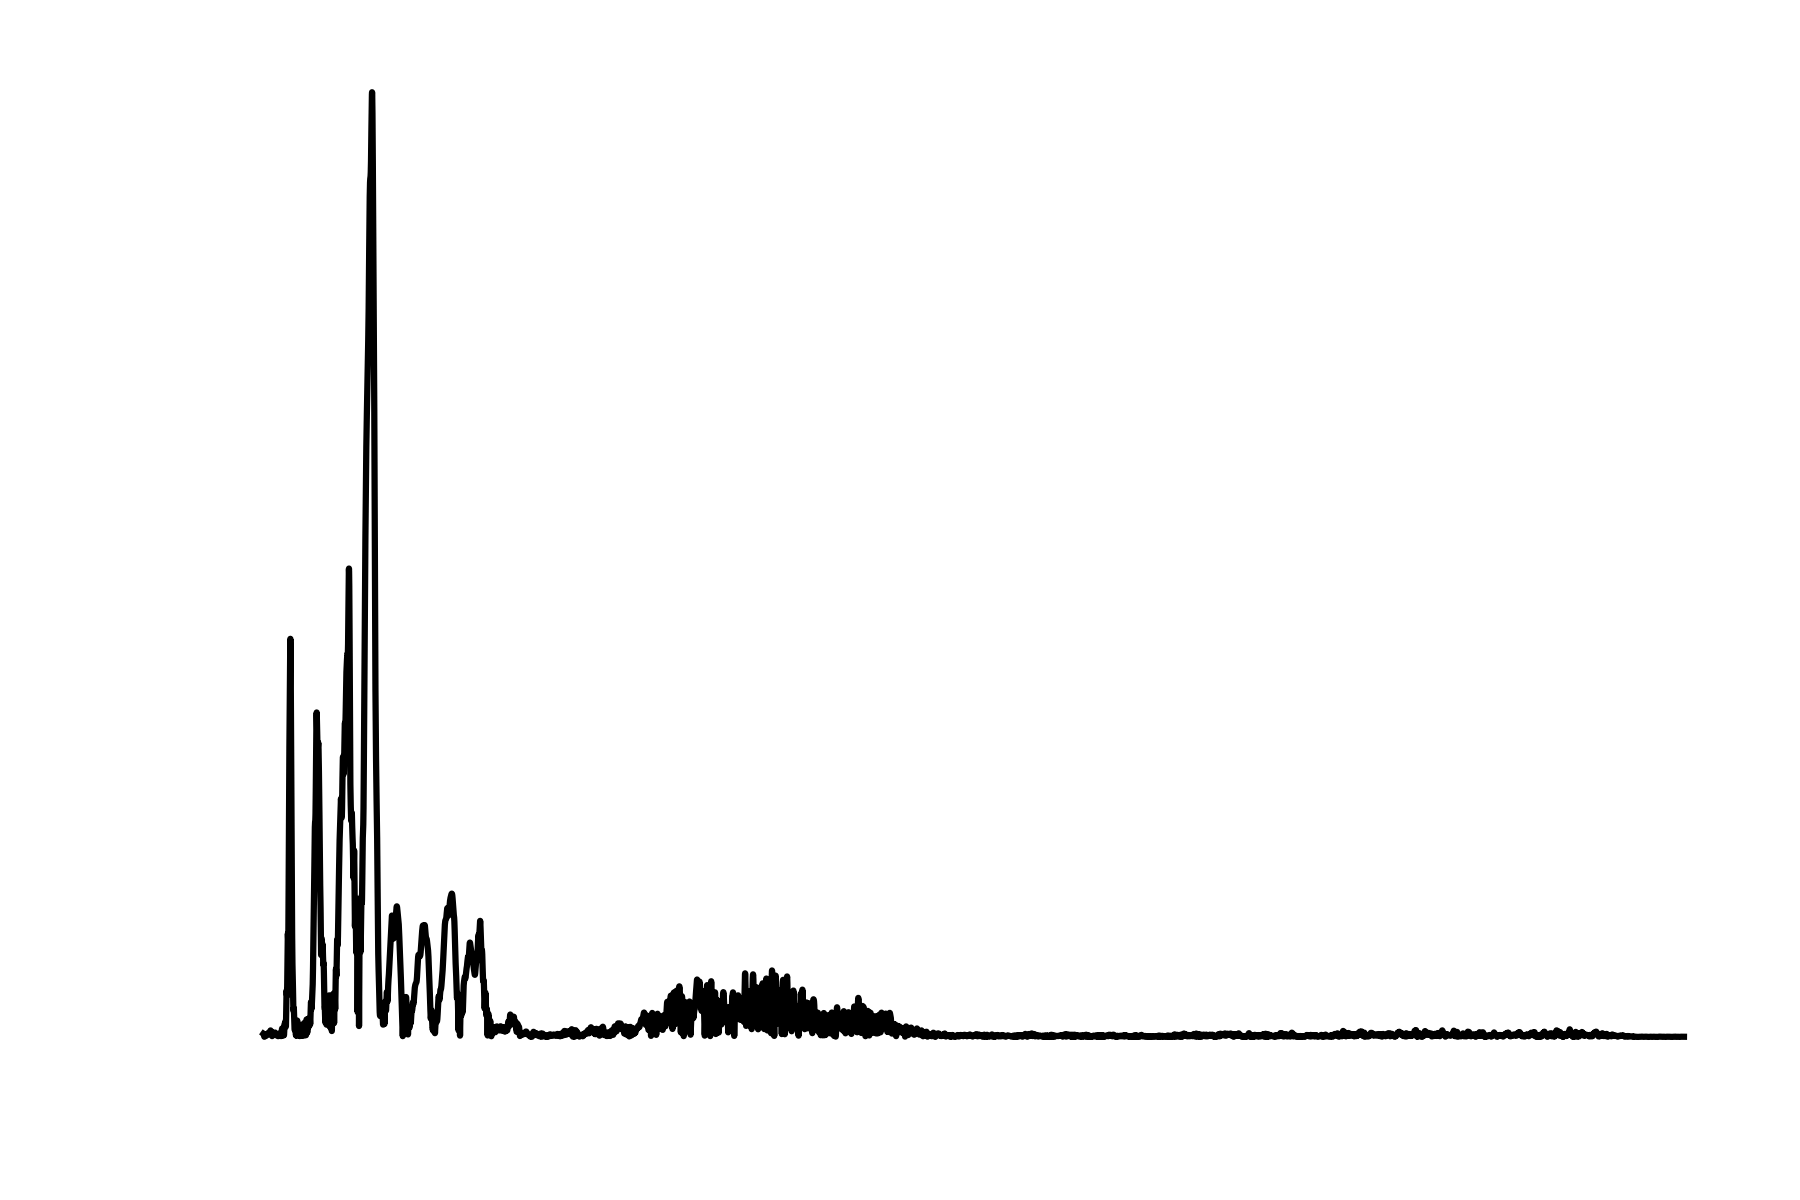
\includegraphics[width=52.5pt,height=35pt]{processing/py-freq_segment-0.png}};
        %Image [id:dp3443235626087914]
        \draw (436,183.33) node  {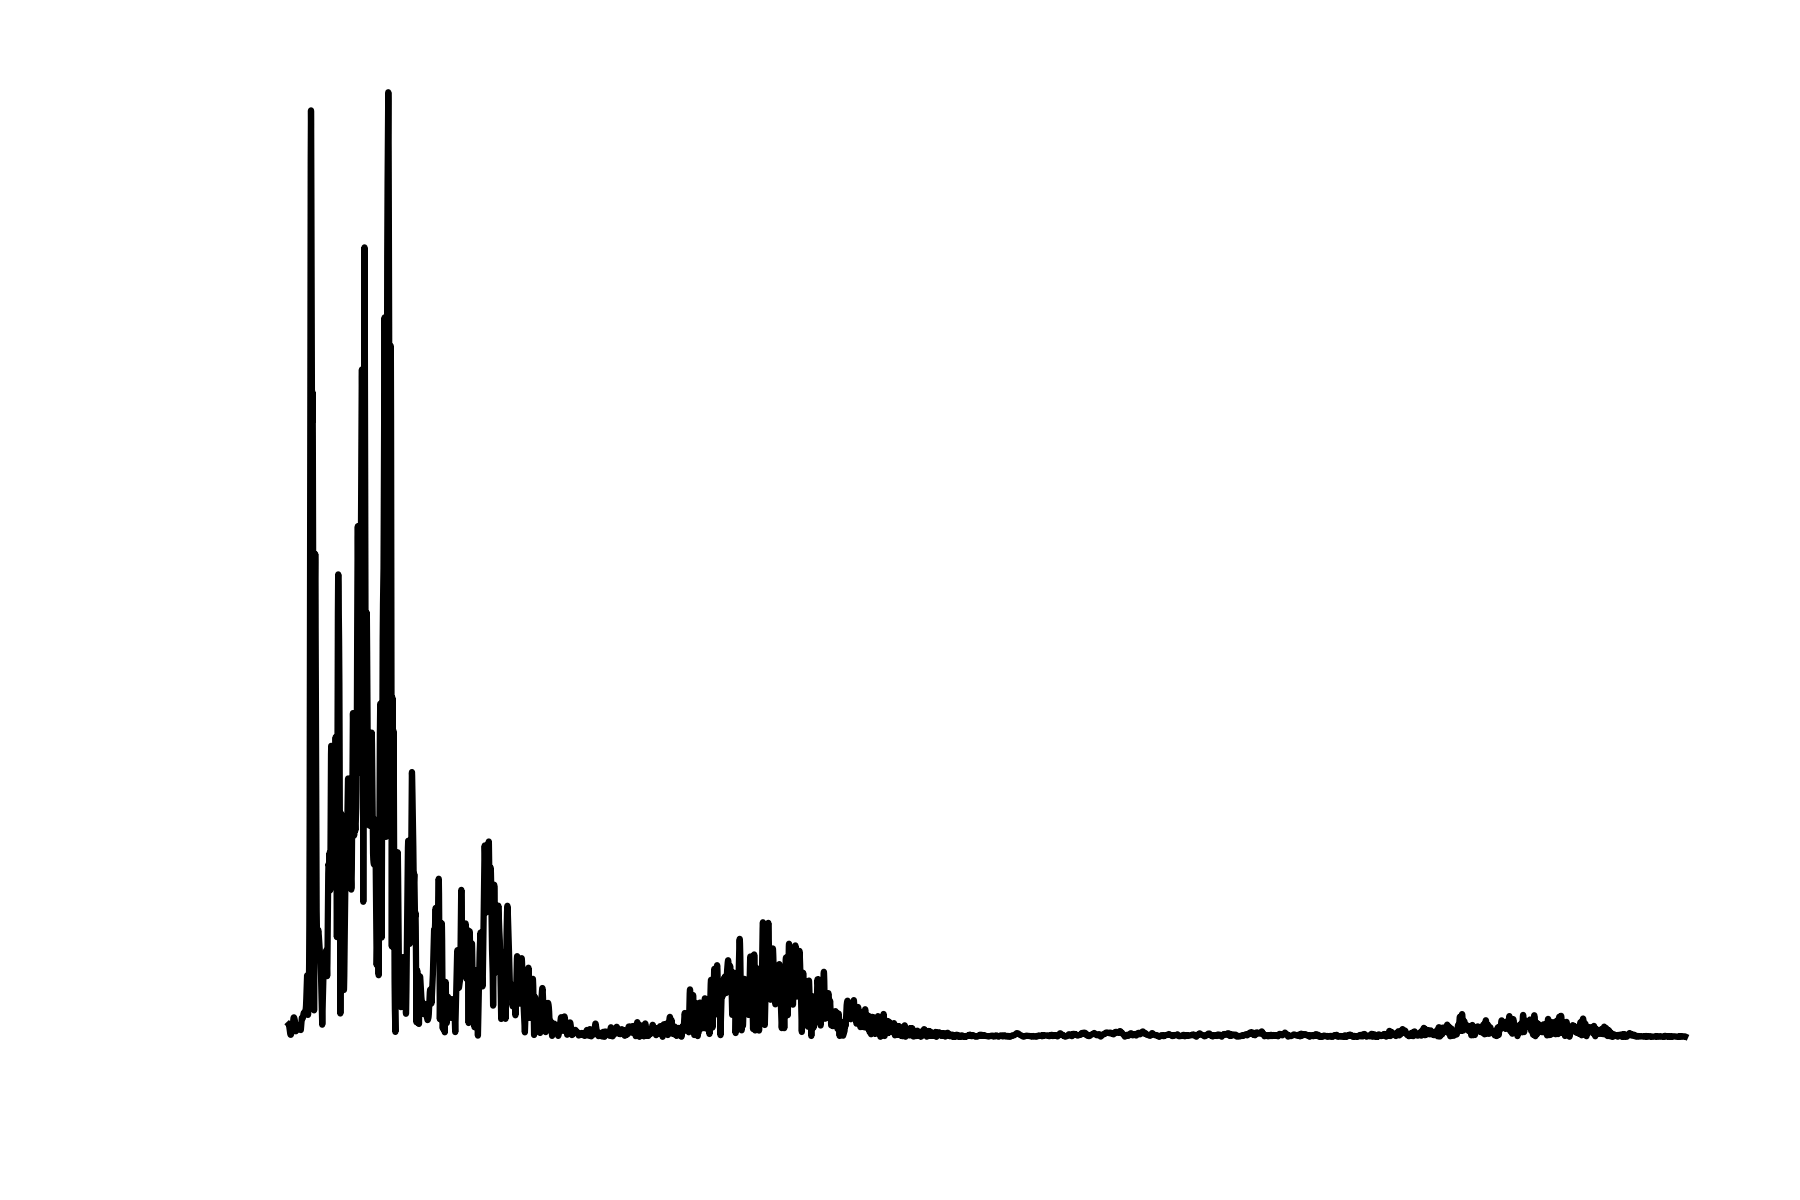
\includegraphics[width=52.5pt,height=35pt]{processing/py-freq_segment-1.png}};
        %Image [id:dp2979363128108309]
        \draw (110,146.5) node  {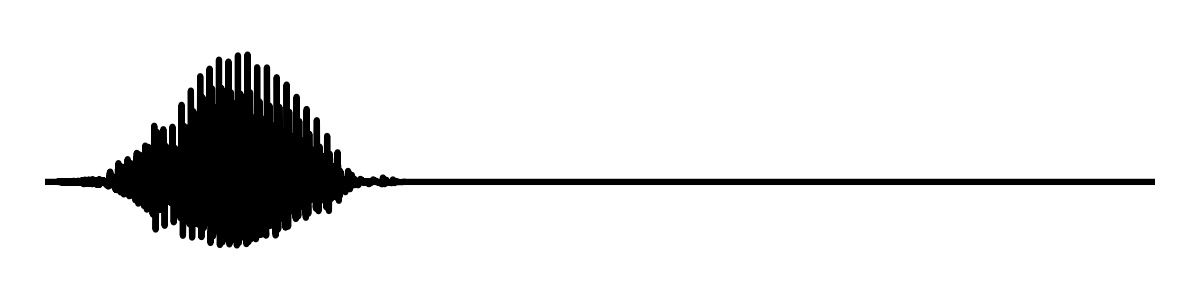
\includegraphics[width=105pt,height=26.25pt]{processing/py-time_segment-0.png}};
        %Shape: Rectangle [id:dp4336148771055519]
        \draw  [draw opacity=0][fill={rgb, 255:red, 255; green, 255; blue, 255 }  ,fill opacity=1 ] (60,180) -- (80,180) -- (80,200) -- (60,200) -- cycle ;
        %Image [id:dp32871739431752567]
        \draw (110,167) node  {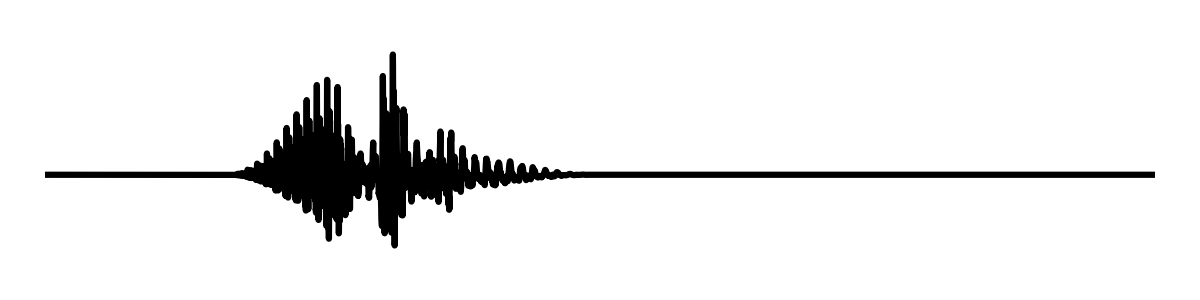
\includegraphics[width=105pt,height=30pt]{processing/py-time_segment-1.png}};
        %Shape: Rectangle [id:dp8481412253766418]
        \draw  [draw opacity=0][fill={rgb, 255:red, 255; green, 255; blue, 255 }  ,fill opacity=1 ] (40,160) -- (60,160) -- (60,200) -- (40,200) -- cycle ;
        %Shape: Rectangle [id:dp03992819043895124]
        \draw  [draw opacity=0][fill={rgb, 255:red, 255; green, 255; blue, 255 }  ,fill opacity=1 ] (120,140) -- (180,140) -- (180,180) -- (120,180) -- cycle ;
        %Image [id:dp2476506667174908]
        \draw (156.75,50.81) node  {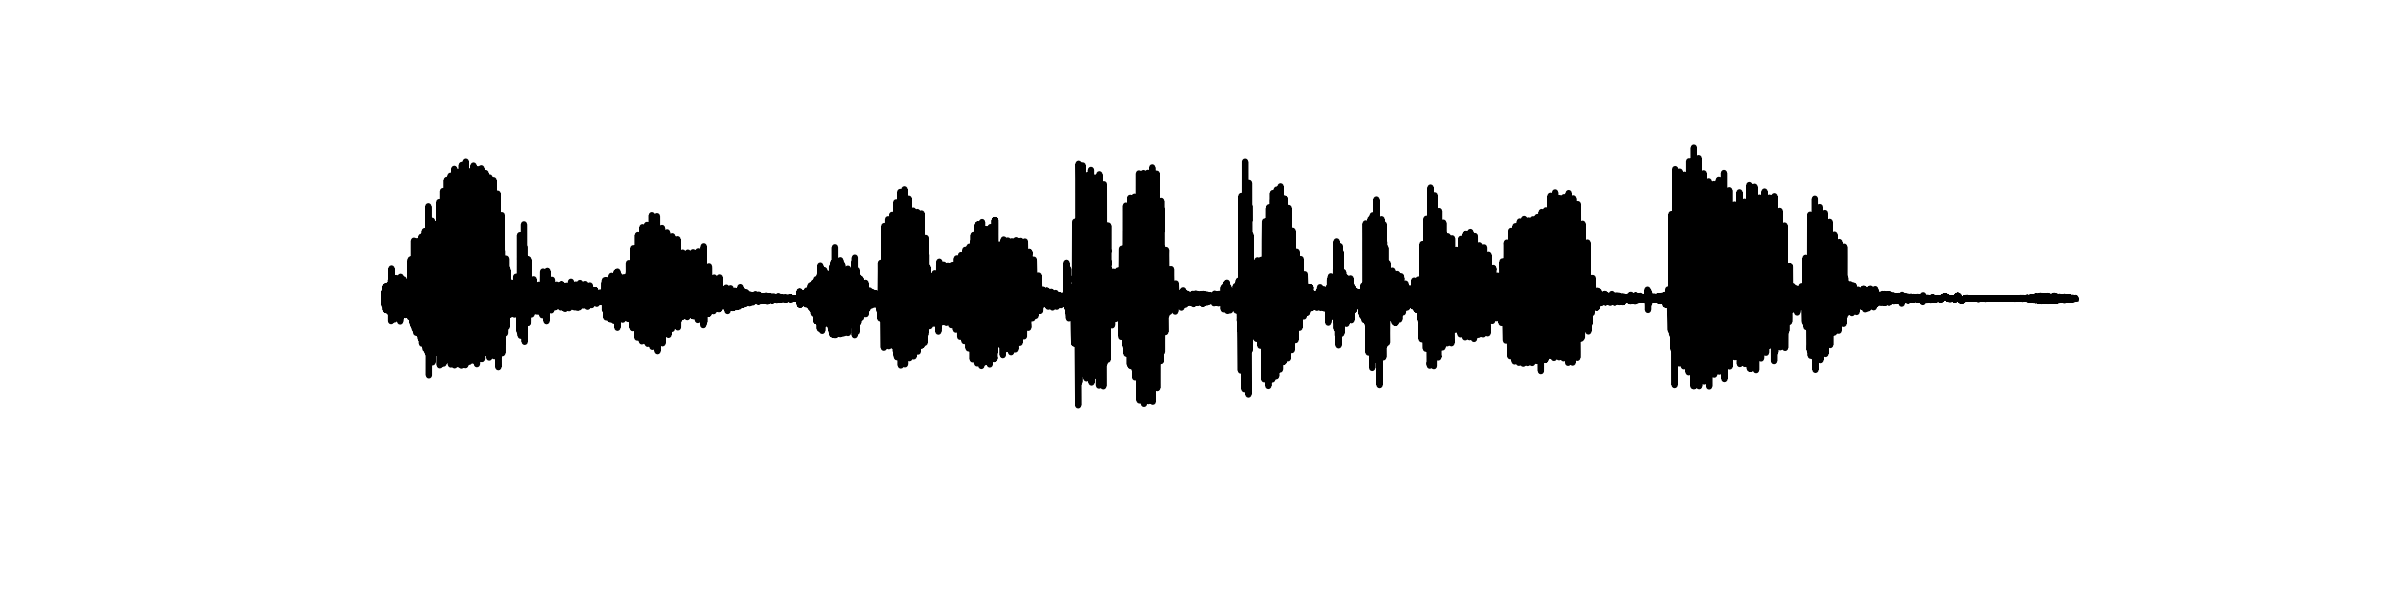
\includegraphics[width=244.88pt,height=61.22pt]{processing/py-waveform.png}};
        %Shape: Rectangle [id:dp29156630749780055]
        \draw  [draw opacity=0][fill={rgb, 255:red, 255; green, 255; blue, 255 }  ,fill opacity=1 ] (160,20) -- (280,20) -- (280,70) -- (160,70) -- cycle ;
        %Image [id:dp4043877940980434]
        \draw (385,130) node  {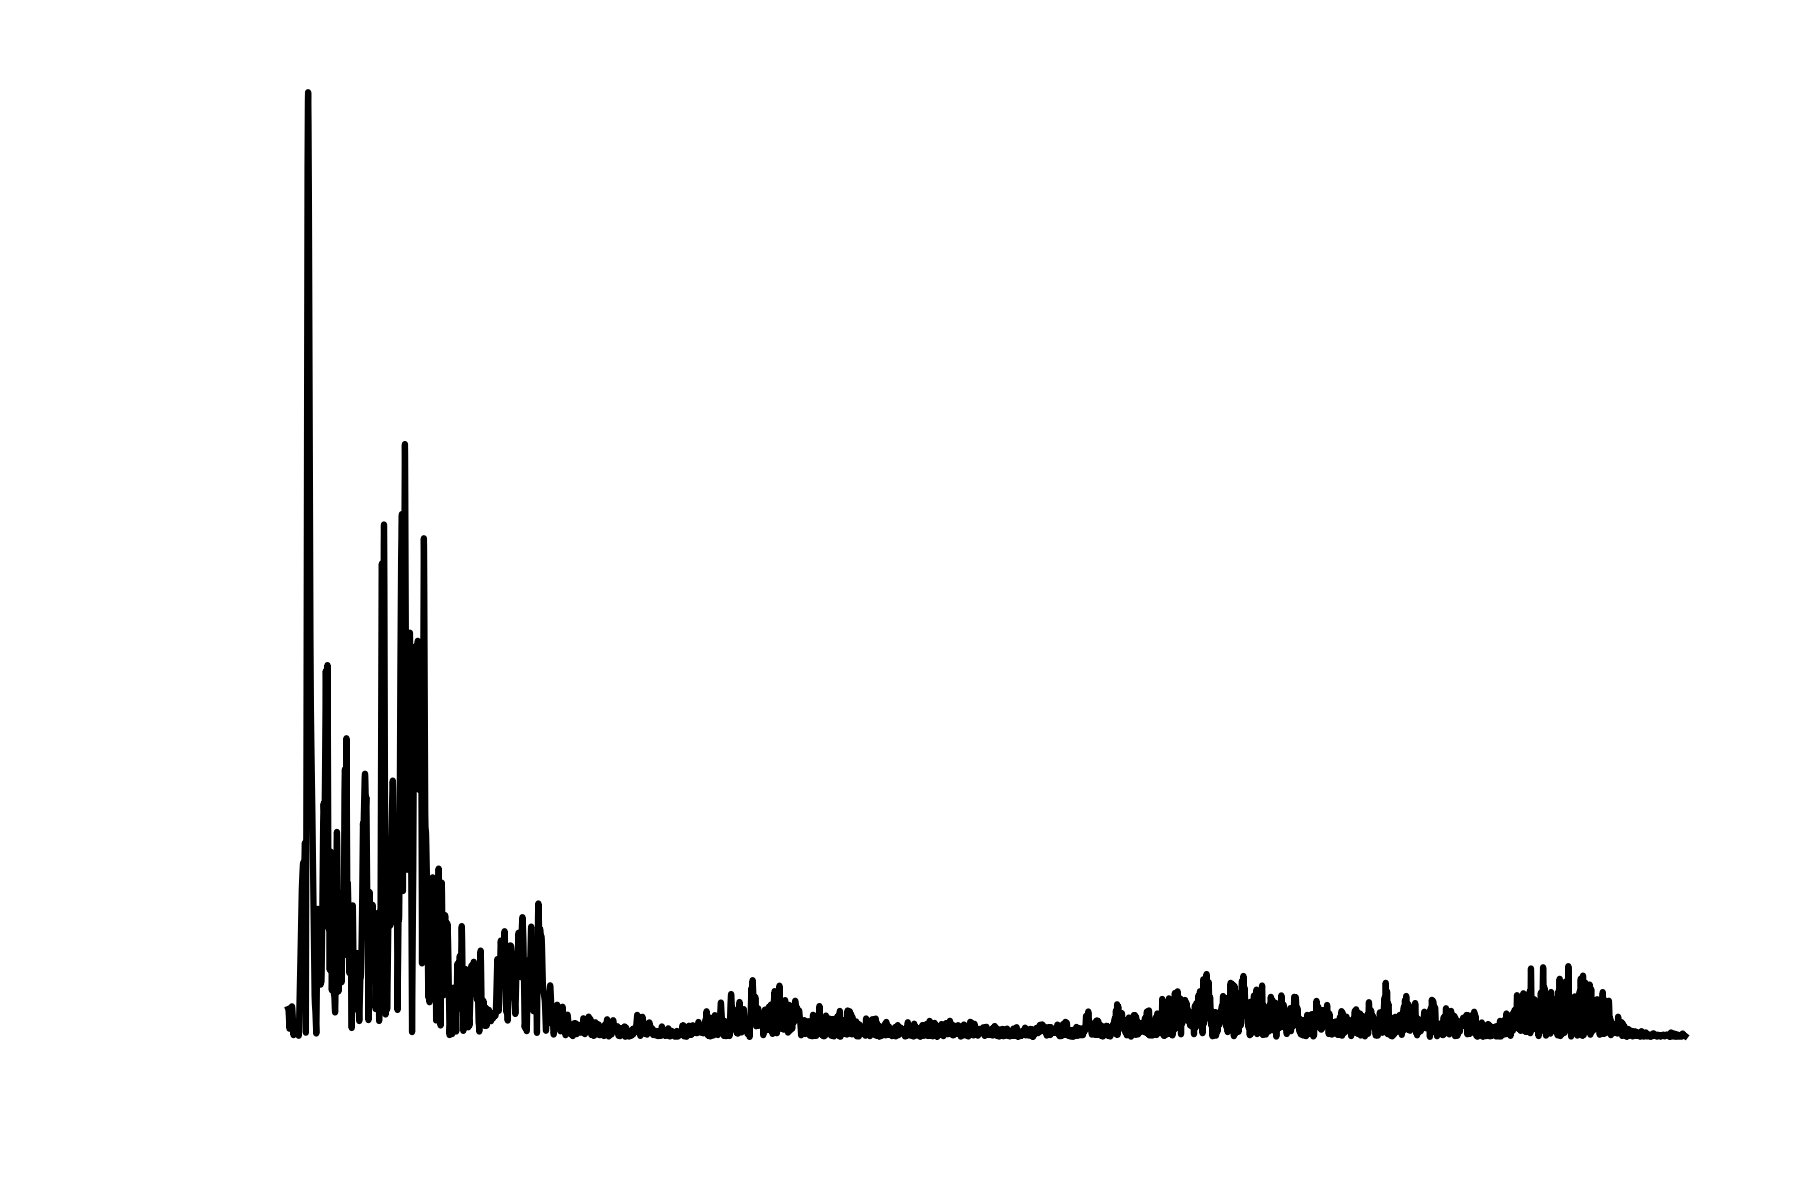
\includegraphics[width=67.5pt,height=45pt]{processing/py-freq_segment-2.png}};
        %Shape: Rectangle [id:dp26622297727772126]
        \draw  [draw opacity=0][fill={rgb, 255:red, 255; green, 255; blue, 255 }  ,fill opacity=1 ] (100,140) -- (120,140) -- (120,160) -- (100,160) -- cycle ;
        %Image [id:dp8105828866624712]
        \draw (105,198.5) node  {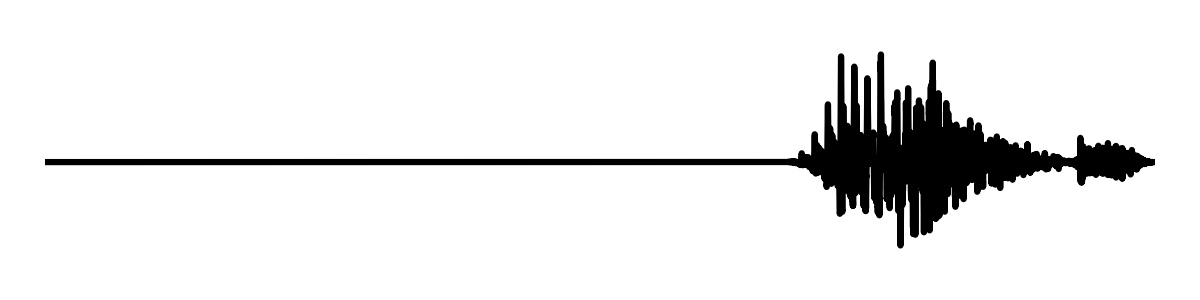
\includegraphics[width=105pt,height=26.25pt]{processing/py-time_segment-2.png}};
        %Shape: Rectangle [id:dp6067652569911224]
        \draw  [draw opacity=0][fill={rgb, 255:red, 255; green, 255; blue, 255 }  ,fill opacity=1 ] (40,190) -- (120,190) -- (120,210) -- (40,210) -- cycle ;
        %Straight Lines [id:da9676641234627033]
        \draw    (130,150) -- (328,150) ;
        \draw [shift={(330,150)}, rotate = 180] [color={rgb, 255:red, 0; green, 0; blue, 0 }  ][line width=0.75]    (4.37,-1.32) .. controls (2.78,-0.56) and (1.32,-0.12) .. (0,0) .. controls (1.32,0.12) and (2.78,0.56) .. (4.37,1.32)   ;
        %Straight Lines [id:da16098226613158673]
        \draw    (150,170) -- (348,170) ;
        \draw [shift={(350,170)}, rotate = 180] [color={rgb, 255:red, 0; green, 0; blue, 0 }  ][line width=0.75]    (4.37,-1.32) .. controls (2.78,-0.56) and (1.32,-0.12) .. (0,0) .. controls (1.32,0.12) and (2.78,0.56) .. (4.37,1.32)   ;
        %Straight Lines [id:da11005264782971791]
        \draw    (190,200) -- (388,200) ;
        \draw [shift={(390,200)}, rotate = 180] [color={rgb, 255:red, 0; green, 0; blue, 0 }  ][line width=0.75]    (4.37,-1.32) .. controls (2.78,-0.56) and (1.32,-0.12) .. (0,0) .. controls (1.32,0.12) and (2.78,0.56) .. (4.37,1.32)   ;
        %Shape: Square [id:dp8422681084136312]
        \draw  [fill={rgb, 255:red, 74; green, 144; blue, 226 }  ,fill opacity=1 ] (370,60) -- (380,60) -- (380,70) -- (370,70) -- cycle ;
        %Shape: Square [id:dp6895251706790707]
        \draw  [fill={rgb, 255:red, 248; green, 231; blue, 28 }  ,fill opacity=1 ] (370,30) -- (380,30) -- (380,40) -- (370,40) -- cycle ;
        %Shape: Square [id:dp8371453826772035]
        \draw  [fill={rgb, 255:red, 245; green, 166; blue, 35 }  ,fill opacity=1 ] (370,20) -- (380,20) -- (380,30) -- (370,30) -- cycle ;
        %Shape: Square [id:dp4704612801462672]
        \draw  [fill={rgb, 255:red, 208; green, 2; blue, 27 }  ,fill opacity=1 ] (370,10) -- (380,10) -- (380,20) -- (370,20) -- cycle ;
        %Shape: Square [id:dp04259158217783243]
        \draw  [fill={rgb, 255:red, 248; green, 231; blue, 28 }  ,fill opacity=1 ] (390,10) -- (400,10) -- (400,20) -- (390,20) -- cycle ;
        %Shape: Square [id:dp8235422331679458]
        \draw  [fill={rgb, 255:red, 80; green, 227; blue, 194 }  ,fill opacity=1 ] (390,20) -- (400,20) -- (400,30) -- (390,30) -- cycle ;
        %Shape: Square [id:dp7304739651989954]
        \draw  [fill={rgb, 255:red, 128; green, 128; blue, 128 }  ,fill opacity=1 ] (390,30) -- (400,30) -- (400,40) -- (390,40) -- cycle ;
        %Shape: Square [id:dp4388945574586607]
        \draw  [fill={rgb, 255:red, 80; green, 227; blue, 194 }  ,fill opacity=1 ] (390,60) -- (400,60) -- (400,70) -- (390,70) -- cycle ;
        %Shape: Square [id:dp9653722203138573]
        \draw  [fill={rgb, 255:red, 248; green, 231; blue, 28 }  ,fill opacity=1 ] (430,30) -- (440,30) -- (440,40) -- (430,40) -- cycle ;
        %Shape: Square [id:dp981513589679916]
        \draw  [fill={rgb, 255:red, 208; green, 2; blue, 27 }  ,fill opacity=1 ] (430,20) -- (440,20) -- (440,30) -- (430,30) -- cycle ;
        %Shape: Square [id:dp8950073186581587]
        \draw  [fill={rgb, 255:red, 189; green, 16; blue, 224 }  ,fill opacity=1 ] (430,10) -- (440,10) -- (440,20) -- (430,20) -- cycle ;
        %Shape: Square [id:dp1665737624049748]
        \draw  [fill={rgb, 255:red, 126; green, 211; blue, 33 }  ,fill opacity=1 ] (430,60) -- (440,60) -- (440,70) -- (430,70) -- cycle ;

        %Straight Lines [id:da7233973673270127]
        \draw    (70,70) -- (70,118) ;
        \draw [shift={(70,120)}, rotate = 270] [color={rgb, 255:red, 0; green, 0; blue, 0 }  ][line width=0.75]    (4.37,-1.32) .. controls (2.78,-0.56) and (1.32,-0.12) .. (0,0) .. controls (1.32,0.12) and (2.78,0.56) .. (4.37,1.32)   ;
        %Image [id:dp28750918753581267]
        \draw (128,113.25) node  {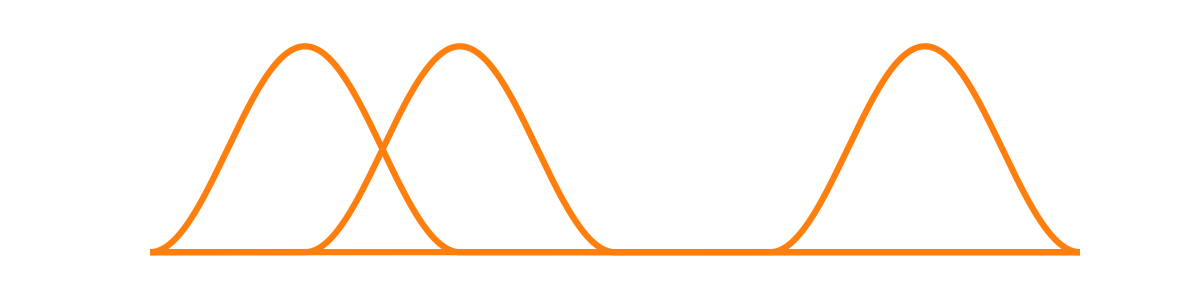
\includegraphics[width=87pt,height=10.13pt]{processing/py-windows.png}};
        %Straight Lines [id:da6893975030077206]
        \draw    (180,50) -- (338,50) ;
        \draw [shift={(340,50)}, rotate = 180] [color={rgb, 255:red, 0; green, 0; blue, 0 }  ][line width=0.75]    (4.37,-1.32) .. controls (2.78,-0.56) and (1.32,-0.12) .. (0,0) .. controls (1.32,0.12) and (2.78,0.56) .. (4.37,1.32)   ;
        %Straight Lines [id:da7882799041842373]
        \draw    (375,140) -- (375,92) ;
        \draw [shift={(375,90)}, rotate = 450] [color={rgb, 255:red, 0; green, 0; blue, 0 }  ][line width=0.75]    (4.37,-1.32) .. controls (2.78,-0.56) and (1.32,-0.12) .. (0,0) .. controls (1.32,0.12) and (2.78,0.56) .. (4.37,1.32)   ;
        %Straight Lines [id:da0855776778601487]
        \draw    (395,160) -- (395,92) ;
        \draw [shift={(395,90)}, rotate = 450] [color={rgb, 255:red, 0; green, 0; blue, 0 }  ][line width=0.75]    (4.37,-1.32) .. controls (2.78,-0.56) and (1.32,-0.12) .. (0,0) .. controls (1.32,0.12) and (2.78,0.56) .. (4.37,1.32)   ;
        %Straight Lines [id:da12659425796956003]
        \draw    (435,190) -- (435,92) ;
        \draw [shift={(435,90)}, rotate = 450] [color={rgb, 255:red, 0; green, 0; blue, 0 }  ][line width=0.75]    (4.37,-1.32) .. controls (2.78,-0.56) and (1.32,-0.12) .. (0,0) .. controls (1.32,0.12) and (2.78,0.56) .. (4.37,1.32)   ;

        % Text Node
        \draw (267.74,169.4) node [anchor=north west][inner sep=0.75pt]  [font=\tiny,rotate=-45.3]  {$\dotsc $};
        % Text Node
        \draw (124,99.4) node [anchor=north west][inner sep=0.75pt]  [font=\footnotesize,color={rgb, 255:red, 245; green, 166; blue, 35 }  ,opacity=1 ]  {$\dotsc $};
        % Text Node
        \draw (241,37) node [anchor=north west][inner sep=0.75pt]  [font=\scriptsize] [align=left] {STFT};
        % Text Node
        \draw (228,137) node [anchor=north west][inner sep=0.75pt]  [font=\scriptsize] [align=left] {DFT};
        % Text Node
        \draw (248,157) node [anchor=north west][inner sep=0.75pt]  [font=\scriptsize] [align=left] {DFT};
        % Text Node
        \draw (271,187) node [anchor=north west][inner sep=0.75pt]  [font=\scriptsize] [align=left] {DFT};
        % Text Node
        \draw (377,126) node [anchor=north west][inner sep=0.75pt]  [font=\tiny,rotate=-270] [align=left] {Vector};
        % Text Node
        \draw (397,126) node [anchor=north west][inner sep=0.75pt]  [font=\tiny,rotate=-270] [align=left] {Vector};
        % Text Node
        \draw (437,126) node [anchor=north west][inner sep=0.75pt]  [font=\tiny,rotate=-270] [align=left] {Vector};
        % Text Node
        \draw (73,111.4) node [anchor=north west][inner sep=0.75pt]  [font=\tiny,color={rgb, 255:red, 245; green, 166; blue, 35 }  ,opacity=1 ]  {$\times $};
        % Text Node
        \draw (401,22.4) node [anchor=north west][inner sep=0.75pt]    {$\dotsc $};
        % Text Node
        \draw (421.4,61) node [anchor=north west][inner sep=0.75pt]  [rotate=-270]  {$\dotsc $};
        % Text Node
        \draw (381.4,61) node [anchor=north west][inner sep=0.75pt]  [rotate=-270]  {$\dotsc $};
        % Text Node
        \draw (361.4,61) node [anchor=north west][inner sep=0.75pt]  [rotate=-270]  {$\dotsc $};


        \end{tikzpicture}


    \end{fullwidthfig}
\end{figure}


\subsection{The final model}
The model \eqref{eq:processing:discreteModel} shows how in practice the RIRs are threated in the frequency-domain.
However this does not generalize straightforwardly to the time-frequency domain:
it depends on the length of the filter \wrt/ to the length of the analysis window on of the \STFT/.
Issues arise with ``long'' filters, which are common in highly reverberant or time-varying scenarios.
To circumvent this issues, the \textit{convolutional STFT} for arbitrary window functions have been proposed\sidenote{%
It translates the time-domain convolution into inter-frame and inter-band convolutions, rather than pointwise multiplication of Fourier transforms.
}~\citeonly{gilloire1992adaptive}.
Although mathematically exact, it is computationally and memory intensive.

In this thesis, we will assume that the filter length is shorter than the analysis window length.
This known in the literature as the \textit{narrowband approximation}, namely the time-domain filtering can be approximated by complex-valued multiplication in each time-frequency bin $[l,k]$:
\begin{equation}
    \imgs_j[l,k] \approx \bsh[k] \src_j[l,k]
    ,
\end{equation}
where the $\bsh_j(f) = \ktranspose{\klist{h_{1j}(f), \cdots, h_{Ij}(f)}}$ is the $I \times 1$ vector of the room transfer functions for the source $j$.
It is sometimes practical to concatenate all this vectors into an $I \times J$ matrix $\bfH(f) = \klist{\bsh_1(f),\cdots,\bsh_J(f)}$ called \textit{mixing matrix}.

With the above notation and considerations, mixing process including noise terms can be written in the \STFT/ domain compactly as:
\begin{equation}\label{eq:processing:model:stfs}
    \bsx[l,k] = \bfH[l,k] \bss[l,k] + \bsu[l,k]
\end{equation}
where $\bsu(l,k) = \bsn(l,k) + \boldsymbol{\varepsilon}(l,k)$ includes the contribution of both diffuse noise sources, modeling and measurement errors.

% The above equation can be seen as a \textit{deterministic} parametrization of the mixing process and it does not consider a statistical description
% of the reverberation. In fact it the filter

% \newthoughtpar{The spatial quadratic STFT transform}
% \begin{equation}
%     \cov_{\mics}[l,k] = \bbE \klist{\mics[l,k]\khermitian{\mics[l,k]}}
% \end{equation}

\section{Other (room) impulse response spectral models}
\RIRs/ are complicated quantities to model, embed in processing frameworks, compute and estimate.
The representations of the \RIR/ discussed so far explicitly model early echoes e reverberation deterministically.
Furthermore, alternative models are common in the audio processing literature.

\subsection{Steering vector model}
In case of absence of echoes and reverberation, namely assuming free-field propagation,
the \RIRs/ simplify to \textit{steering vector}, namely the DFT of~\cref{eq:acoustics:greenFreeTime}:
\begin{equation}\label{eq:processing:steering}
    \bsd_{j}[k] = \klist{\frac{1}{4 \pi \distMicSrc_{1j}} \cste^{-\csti 2 \pi f_k \distMicSrc_{1j} / c},
                            \cdots,
                            \frac{1}{4 \pi \distMicSrc_{Ij}} \cste^{-\csti 2 \pi f_k \distMicSrc_{Ij} / c},
                    }
\end{equation}
Furthermore, assuming far-field regimes, the microphone-to-source distance $\distMicSrc_{ij}$ are larger than the
inter-microphones distance $d_{ii'}$ making the attenuation factors $\sfrac{1}{4 \pi \distMicSrc_{ij}}$ approximately equal, hence ignored.

\subsection{Relative transfer function and interchannel models}
Let us consider now only two channels and only one source signal in the model~\cref{eq:processing:model:stfs}.
Dropping the dependency on $j$ for readability and taking the first channel as reference, the \RTFdef/ associated the the $i$-th channel is defined as
the element-wise ratio of the (D)FTs of the two filters~\citeonly{gannot2001signal}
\begin{equation}\label{eq:processing:rtf}
    \rtf_i[k] = \frac{\rir_i[k]}{\rir_1[k]}
    .
\end{equation}

The time-domain counterpart is called as \ReIRdef/ and can be interpreted as the filter ``transforming'' the $i$-th impulse response into the one of the reference channel.
Considering the noisy observation $x_i$ and $x_1$, their signals can be re-written in term of $\rtf_i$ as follows
\begin{equation}
    \begin{matrix}
    \begin{cases}
        \mic_1 = \rir_1 \conv s + \allNoise_1 \\
        \mic_i = \rir_i \conv s + \allNoise_i
    \end{cases} & \kto  & \begin{cases}
        \mic_1 = \rir_1 \conv s + \allNoise_1 \\
        \mic_i = \rtf_i \conv \rir_i \conv s + \allNoise_i
    \end{cases}
    \end{matrix}
    .
\end{equation}
Notice that $\rir_i = \rtf_i \conv \rir_1$, corresponding to~\cref{eq:processing:rtf} in the frequency domain.
Moreover although the real-world \RIRs/ $h_1$ and $h_i$ are causal, their \RTF/ need not be so.
\marginpar{%
    \footnotesize
    In~\cref{ch:brioche} methods for estimation the RTF will be discussed
}

The \RTFs/ benefits of several interesting properties that will be of fundamental importance for this thesis.
In particular:
\begin{itemize}
    \item the \RTF/ associated to the reference channel ($i = 1$) is equal to $1$ for each frequency bin $k$.
    \item The problem of estimating the \RTF/ can be considered ``easier'' with respect to the \RIRs/ estimation.
    In fact, in noiseless case, it holds that $\mic_i = \rtf_i \conv \mic_1$.
    \item The \RTF/ encodes properties of the related impulse responses and there are many advance methods to estimate them.
    Therefore, it may be used as a proxy for the estimations of (components of) \RIRs/.
    \item A \RIR/ can be seen as a special case of \RTF/ where the non-reference microphone is a virtual one whose
    output is the original (non-spatial) source signal $\src$. In fact, if $\rir_1 = \delta$ then $\rtf_i = \rir_i$\sidenote{%
    In practice this virtual microphone is substituted by a microphone that is very close to the source.}.
    \item As discussed below, also \RTFs/ simplify to special steering vectors in free- and far-field, which has interesting
    geometrical properties.
\end{itemize}

In the general case of multiple microphone array ($I>2$) and multiple sources, the vector of \RTFs/ $\rtfs_j[k] = \ktranspose{\klist{\rtf_ {1j}, \cdots, \rtf_{Ij}}}$
for the $j$-th source is defined as
\begin{equation}\label{eq:processing:rtf}
    \rtfs_j[k] = \frac{1}{\rir_{1j}[k]} \rirs_j[k]
    .
\end{equation}


\newthought{The relative steering vectors} results by combining~\cref{eq:processing:steering,eq:processing:rtf} as
\begin{equation}
    \boldsymbol{\tilde{d}}_{j}[k] = \klist{
                         1,
                         \cste^{-\csti 2 \pi f_k (\distMicSrc_{2j}-\distMicSrc_{i'j}) / \speedOfSound},
                         \cdots,
                         \cste^{-\csti 2 \pi f_k (\distMicSrc_{Ij}-\distMicSrc_{i'j}) / \speedOfSound},
                    }
\end{equation}
where $\sfrac{(\distMicSrc_{ij}-\distMicSrc_{1j})}{\speedOfSound}$ is the \TDOA/ between the $i$-th and the reference microphones.
The \TDOAs/ will be the protagonists of~\cref{chap:mirage} as they are fundamental quantities for sound source localization.

\newthought{In the context of spatial auditory perception} and \CASA/, the \RTF/ is related to the \textit{interchannel cues}\sidenote{%
sometimes refers to as \textit{interaural cues} when a stress is put on the fact that the two ears are considered as receivers}.
In fact, the \RTFs/ encodes the so-called \ILD/ and the \IPD/
\begin{equation}
    \begin{aligned}
        \ild_{ij}[k] &= 20 \log_{10} \magnitudeOf{\rtf[k]} & [\si{\dB}]\\
        \ipd_{ij}[k] &= \phaseOf{\rtf[k]} \mathspace       & [\si{\radian}]
    \end{aligned}
\end{equation}

As shown in~\cref{fig:processing:ildipd}, the \ILD/ and the \IPD/ cluster around the direct path.
However early echoes and reverberation make them significantly diverge.


% \subsection{Probabilistic and Full-rank covariance model}
% For certain applications, it is more common to assume a statistical point of view, known as the \textit{Local Gaussian Model}\cite{}.
% Assume that the source STFT coefficients sj(n, f) have a zero-mean nonstationary Gaussian distribution with variance σ2
% sj (n, f), and they are all independent source-,
% frame- and frequency-wise (i.e., over j, n and f)